\PassOptionsToPackage{unicode=true}{hyperref} % options for packages loaded elsewhere
\PassOptionsToPackage{hyphens}{url}
%
\documentclass[,man,floatsintext]{apa6}
\usepackage{lmodern}
\usepackage{amssymb,amsmath}
\usepackage{ifxetex,ifluatex}
\usepackage{fixltx2e} % provides \textsubscript
\ifnum 0\ifxetex 1\fi\ifluatex 1\fi=0 % if pdftex
  \usepackage[T1]{fontenc}
  \usepackage[utf8]{inputenc}
  \usepackage{textcomp} % provides euro and other symbols
\else % if luatex or xelatex
  \usepackage{unicode-math}
  \defaultfontfeatures{Ligatures=TeX,Scale=MatchLowercase}
\fi
% use upquote if available, for straight quotes in verbatim environments
\IfFileExists{upquote.sty}{\usepackage{upquote}}{}
% use microtype if available
\IfFileExists{microtype.sty}{%
\usepackage[]{microtype}
\UseMicrotypeSet[protrusion]{basicmath} % disable protrusion for tt fonts
}{}
\IfFileExists{parskip.sty}{%
\usepackage{parskip}
}{% else
\setlength{\parindent}{0pt}
\setlength{\parskip}{6pt plus 2pt minus 1pt}
}
\usepackage{hyperref}
\hypersetup{
            pdftitle={A multi-lab study of bilingual infants: Exploring the preference for infant-directed speech},
            pdfauthor={Krista Byers-Heinlein, Angeline Sin Mei Tsui, Christina Bergmann, Alexis Black, Anna Brown, Maria Julia Carbajal, Samantha Durrant, Christopher T. Fennell, Anne-Caroline Fiévet, Michael C. Frank, Anja Gampe, Judit Gervain, Nayeli Gonzalez-Gomez, J. Kiley Hamlin, Naomi Havron, Mikołaj Hernik, Shila Kerr, Hilary Killam, Kelsey Klassen, Jessica Kosie, Ágnes Melinda Kovács, Casey Lew-Williams, Liquan Liu, Nivedita Mani, Caterina Marino, Meghan Mastroberardino, Victoria Mateu, Clarie Noble, Adriel John Orena, Linda Polka, Christine E. Potter, Melanie Schreiner, Leher Singh, Melanie Soderstrom, Megha Sundara, Connor Waddell, Janet F. Werker, \& Stephanie Wermelinger},
            pdfkeywords={language acquisition; bilingualism; speech perception; infant-directed speech; reproducibility; experimental methods},
            pdfborder={0 0 0},
            breaklinks=true}
\urlstyle{same}  % don't use monospace font for urls
\usepackage{graphicx,grffile}
\makeatletter
\def\maxwidth{\ifdim\Gin@nat@width>\linewidth\linewidth\else\Gin@nat@width\fi}
\def\maxheight{\ifdim\Gin@nat@height>\textheight\textheight\else\Gin@nat@height\fi}
\makeatother
% Scale images if necessary, so that they will not overflow the page
% margins by default, and it is still possible to overwrite the defaults
% using explicit options in \includegraphics[width, height, ...]{}
\setkeys{Gin}{width=\maxwidth,height=\maxheight,keepaspectratio}
\setlength{\emergencystretch}{3em}  % prevent overfull lines
\providecommand{\tightlist}{%
  \setlength{\itemsep}{0pt}\setlength{\parskip}{0pt}}
\setcounter{secnumdepth}{0}
% Redefines (sub)paragraphs to behave more like sections
\ifx\paragraph\undefined\else
\let\oldparagraph\paragraph
\renewcommand{\paragraph}[1]{\oldparagraph{#1}\mbox{}}
\fi
\ifx\subparagraph\undefined\else
\let\oldsubparagraph\subparagraph
\renewcommand{\subparagraph}[1]{\oldsubparagraph{#1}\mbox{}}
\fi

% set default figure placement to htbp
\makeatletter
\def\fps@figure{htbp}
\makeatother

\shorttitle{A multi-lab study of bilingual infants}
\affiliation{
\vspace{0.5cm}
\textsuperscript{1} Concordia University\\\textsuperscript{2} Stanford University\\\textsuperscript{3} Max Planck Institute for Psycholinguistics\\\textsuperscript{4} University of British Columbia\\\textsuperscript{5} University of Liverpool\\\textsuperscript{6} ENS, EHESS, CNRS, PSL University\\\textsuperscript{7} University of Ottawa\\\textsuperscript{8} University of Zurich\\\textsuperscript{9} Integrative Neuroscience and Cognition Center (INCC), CNRS \& Université Paris Descartes\\\textsuperscript{10} Oxford Brookes University\\\textsuperscript{11} UiT The Arctic University of Norway\\\textsuperscript{12} McGill University, School of Communication Sciences and Disorders\\\textsuperscript{13} University of Manitoba\\\textsuperscript{14} Princeton University\\\textsuperscript{15} Central European University\\\textsuperscript{16} Western Sydney University\\\textsuperscript{17} UCLA\\\textsuperscript{18} National University of Singapore\\\textsuperscript{19} University of Göttingen}
\keywords{language acquisition; bilingualism; speech perception; infant-directed speech; reproducibility; experimental methods\newline\indent Word count: 13054}
\usepackage{csquotes}
\usepackage{upgreek}
\captionsetup{font=singlespacing,justification=justified}

\usepackage{longtable}
\usepackage{lscape}
\usepackage{multirow}
\usepackage{tabularx}
\usepackage[flushleft]{threeparttable}
\usepackage{threeparttablex}

\newenvironment{lltable}{\begin{landscape}\begin{center}\begin{ThreePartTable}}{\end{ThreePartTable}\end{center}\end{landscape}}

\makeatletter
\newcommand\LastLTentrywidth{1em}
\newlength\longtablewidth
\setlength{\longtablewidth}{1in}
\newcommand{\getlongtablewidth}{\begingroup \ifcsname LT@\roman{LT@tables}\endcsname \global\longtablewidth=0pt \renewcommand{\LT@entry}[2]{\global\advance\longtablewidth by ##2\relax\gdef\LastLTentrywidth{##2}}\@nameuse{LT@\roman{LT@tables}} \fi \endgroup}


\usepackage{lineno}

\linenumbers
\usepackage{amsmath}

\title{A multi-lab study of bilingual infants: Exploring the preference for infant-directed speech}
\author{Krista Byers-Heinlein\textsuperscript{1}, Angeline Sin Mei Tsui\textsuperscript{2}, Christina Bergmann\textsuperscript{3}, Alexis Black\textsuperscript{4}, Anna Brown\textsuperscript{5}, Maria Julia Carbajal\textsuperscript{6}, Samantha Durrant\textsuperscript{5}, Christopher T. Fennell\textsuperscript{7}, Anne-Caroline Fiévet\textsuperscript{6}, Michael C. Frank\textsuperscript{2}, Anja Gampe\textsuperscript{8}, Judit Gervain\textsuperscript{9}, Nayeli Gonzalez-Gomez\textsuperscript{10}, J. Kiley Hamlin\textsuperscript{4}, Naomi Havron\textsuperscript{6}, Mikołaj Hernik\textsuperscript{11}, Shila Kerr\textsuperscript{12}, Hilary Killam\textsuperscript{1}, Kelsey Klassen\textsuperscript{13}, Jessica Kosie\textsuperscript{14}, Ágnes Melinda Kovács\textsuperscript{15}, Casey Lew-Williams\textsuperscript{14}, Liquan Liu\textsuperscript{16}, Nivedita Mani\textsuperscript{19}, Caterina Marino\textsuperscript{9}, Meghan Mastroberardino\textsuperscript{1}, Victoria Mateu\textsuperscript{17}, Clarie Noble\textsuperscript{5}, Adriel John Orena\textsuperscript{12}, Linda Polka\textsuperscript{12}, Christine E. Potter\textsuperscript{14}, Melanie Schreiner\textsuperscript{19}, Leher Singh\textsuperscript{18}, Melanie Soderstrom\textsuperscript{13}, Megha Sundara\textsuperscript{17}, Connor Waddell\textsuperscript{16}, Janet F. Werker\textsuperscript{4}, \& Stephanie Wermelinger\textsuperscript{8}}
\date{}

\authornote{``Individual participating labs acknowledge funding support from: the Natural Sciences and Engineering Research Council of Canada (402470-2011 and 2015-03967); the Social Sciences and Humanities Research Council of Canada Insight Grant (435-2015-1974 and 435-2015-0385); Agence Nationale de la Recherche (ANR-17-EURE-0017 and ANR-10-IDEX-0001-02); Western Sydney University Early Career Researcher Start-up Grant (20311.87608); European Commission (MSCA-IF-798658); a European Research Council Synergy Grant, SOMICS (609819); ERC Consolidator Grant''BabyRhythm" (773202); The Leverhulme Trust (ECF-2015-009); The UK Economic and Social Research Council (ES/L008955/1); Research Manitoba, Children's Hospital Research Institute of Manitoba, University of Manitoba; ODPRT funds, National University fo Singapore; and the National Institute of Child Health and Human Development (R01HD095912)."

Correspondence concerning this article should be addressed to Krista Byers-Heinlein, 7141 Sherbrooke St.~West, Montreal, QC, H4B 1R6, Canada. E-mail: \href{mailto:k.byers@concordia.ca}{\nolinkurl{k.byers@concordia.ca}}}

\abstract{
From the earliest months of life, infants prefer listening to and learn better from infant-directed speech (IDS) than adult-directed speech (ADS). Yet, IDS differs within communities, across languages, and across cultures, both in form and in prevalence. This large-scale, multi-site study used the diversity of bilingual infant experiences to explore the impact of different types of linguistic experience on infants' IDS preference. As part of the multi-lab ManyBabies project, we compared lab-matched samples of 333 bilingual and 385 monolingual infants' preference for North-American English IDS (cf.~ManyBabies Consortium, in press (MB1)), tested in 17 labs in 7 countries. Those infants were tested in two age groups: 6--9 months (the younger sample) and 12--15 months (the older sample). We found that bilingual and monolingual infants both preferred IDS to ADS, and did not differ in terms of the overall magnitude of this preference. However, amongst bilingual infants who were acquiring North-American English (NAE) as a native language, greater exposure to NAE was associated with a stronger IDS preference, extending the previous finding from MB1 that monolinguals learning NAE as a native language showed a stronger preference than infants unexposed to NAE. Together, our findings indicate that IDS preference likely makes a similar contribution to monolingual and bilingual development, and that infants are exquisitely sensitive to the nature and frequency of different types of language input in their early environments.


}

\begin{document}
\maketitle

When caregivers interact with their infants, their speech often takes on specific, distinguishing features in a speech register known as infant-directed speech (IDS; Fernald et al., 1989). IDS is produced by caregivers of most (although not all) linguistic and cultural backgrounds, and is typically characterized by a slow, melodic, high-pitched, and exaggerated cadence (Farran, Lee, Yoo, \& Oller, 2016; Fernald et al., 1989; Kitamura, Thanavishuth, Burnham, \& Luksaneeyanawin, 2001; Pye, 1986; Shute \& Wheldall, 1999). From early in life, infants tune their attention to IDS, preferring to listen to IDS over adult-directed speech (ADS) both at birth (Cooper \& Aslin, 1990), as well as later in infancy (Cooper, Abraham, Berman, \& Staska, 1997; Cooper \& Aslin, 1994; Fernald, 1985; Hayashi, Tamekawa, \& Kiritani, 2001; Kitamura \& Lam, 2009; Newman \& Hussain, 2006; Pegg, Werker, \& McLeod, 1992; Santesso, Schmidt, \& Trainor, 2007; Singh, Morgan, \& Best, 2002; Werker \& McLeod, 1989; Werker, Pegg, \& McLeod, 1994).

Infants' preference for IDS may play a useful role in early language learning. For example, infants are better able to discriminate speech sounds in IDS than in ADS (Karzon, 1985; Trainor \& Desjardins, 2002), more efficiently segment words from continuous speech in an IDS register (Thiessen, Hill, \& Saffran, 2005), demonstrate better long-term memory for words spoken in IDS (Singh, Nestor, Parikh, \& Yull, 2009) and learn new words more effectively from IDS than ADS (Graf Estes \& Hurley, 2013; Ma, Golinkoff, Houston, \& Hirsh-Pasek, 2011; but see Schreiner, Altvater-Mackensen, \& Mani, 2016).

While most studies have confirmed a general, early preference for IDS, to date there is very little research aimed at understanding how different linguistic experiences affect infants' preferences. For instance, although the existence of IDS has been demonstrated in a large number of cultures (see above citations), the vast majority of the research on infants' IDS preferences has been conducted in North America, using English speech typically directed at North American English-hearing infants (Dunst, Gorman, \& Hamby, 2012). Most critically, past work has been limited to a particular kind of linguistic (and cultural) experience: that of the monolingual infant. Here, we present a large-scale, multi-site, pre-registered study on bilingual infants, a population that is particularly suited to explore the relationship between language experience and IDS preference. Moreover, this research provides important insight into the early development of bilingual infants, a large but understudied population.

\hypertarget{does-experience-tune-infants-preference-for-ids}{%
\subsection{Does experience tune infants' preference for IDS?}\label{does-experience-tune-infants-preference-for-ids}}

What role might experience play in tuning infants' attention to IDS? We aggregated results from a recent published meta-analysis (Dunst et al., 2012) with additional community-contributed data (MetaLab, 2017) to examine their combined results. When all 62 studies are considered, we found a moderately-sized average effect of Cohen's \(d\) =.64. A focus on the 22 studies most similar to ours (testing IDS preference using looking times collected in a laboratory, among typically-developing infants from 3--15 months, with naturally-produced English-spoken IDS from an unfamiliar female speaker), the effect size is slightly lower, \(d\) = .6. Although this meta-analysis focused on infants in the first year of life, other studies of infants aged 18--21 months have also reported a preference for IDS over ADS (Glenn \& Cunningham, 1983; Robertson, von Hapsburg, \& Hay, 2013). There is some evidence that older infants show a greater preference for IDS than younger infants (Dunst et al., 2012), although an age effect was not found in the subsample of 22 studies mentioned above. More evidence is needed to explore the possibility that increased language experience as children grow enhances their preference for IDS.

Another variable that would be important in understanding the role of experience in the preference for IDS is whether the speech stimuli were presented in a native or non-native language. Numerous studies in early perception find different developmental trajectories for perception of native versus non-native stimuli (e.g.~discriminating human faces vs.~discriminating monkey faces, Lewkowicz \& Ghazanfar, 2006; discriminating native vs.~discriminating non-native speech sound categories, Maurer \& Werker, 2014; segmenting word forms from fluent speech, e.g., Polka \& Sundara, 2012). Generally, whereas infants show increasing proficiency in discriminating the types of faces and sounds that are present in their environment, they lose sensitivity to the differences between non-native stimuli over time. This general pattern might lead us to predict that infants will initially be sensitive to differences between IDS and ADS in both the native and non-native languages, but that this initial cross-linguistic sensitivity will decline with age. In other words, at some ages, infants' preference for IDS over ADS could be enhanced when hearing their native language. However, to date, there is very little data on this question. Importantly, this general trend, if it exists, may interact with differences across languages in the production of IDS. The exaggerated IDS of North American English might be either more interesting or less interesting to an infant whose native language is characterized by a less exaggerated form IDS, than for an infant who regularly hears North American English IDS.

Only a handful of IDS preference studies have explicitly explored infants' preference for IDS from infants' native versus a non-native language. Werker et al. (1994) compared 4.5- and 9-month-old English and Cantonese-learning infants' preference for videos of Cantonese mothers using IDS versus ADS. Both groups showed a preference for IDS; however, the magnitude of the preference between the two groups was not specifically compared (Werker et al., 1994). Hayashi et al. (2001) studied Japanese-learning infants' (aged 4--14 months) preference for native (Japanese) and non-native (English) speech. Japanese-learning infants generally showed a preference for Japanese IDS over ADS, as well as an increasing preference for Japanese IDS over English IDS. The latter finding shows that infants tune into their native language with increased experience; however, as the study did not measure infants' interest in English ADS, we do not know whether Japanese infants were equally sensitive to the difference between ADS and IDS in the non-native stimuli, or whether/how this might change over time.

Infants growing up bilingual are typically exposed to IDS in two languages. They provide a particularly useful wedge in understanding experiential influences on infants' attention to IDS. Bilingual infants receive less exposure to each of their languages than monolingual infants, and the exact proportion of exposure to each of their two languages varies from infant to infant. This divided exposure does not appear to slow the overall rate of language acquisition: bilinguals pass their language milestones on approximately the same schedule as monolingual infants, such as the onset of babbling and the production of their first words (Werker \& Byers-Heinlein, 2008). Nonetheless, children from different language backgrounds receive different types of input, and must ultimately acquire different language forms, which can alter some patterns of language acquisition (e.g., Choi \& Bowerman, 1991; Slobin, 1985; Tardif, 1996; Tardif, Shatz, \& Naigles, 1997; Werker \& Tees, 1984). As a consequence, bilingual infants allow researchers to investigate how a given \enquote{dose} of experience with a specific language relates to phenomena in language acquisition, while holding infants' age and total experience with language constant (Byers-Heinlein \& Fennell, 2014).

Aside from the opportunity to study dose effects, it is important to examine the preference for IDS in bilingual infants for the sake of understanding bilingual development itself. Several lines of research suggest that early exposure to two languages changes some aspects of early development (Byers-Heinlein \& Fennell, 2014), including bilinguals' perception of non-native speech sounds (i.e., sounds that are in neither of their native languages). For example, a number of studies have reported that bilinguals maintain sensitivity to non-native consonant contrasts (García-Sierra, Ramírez-Esparza, \& Kuhl, 2016; Petitto et al., 2012; Ramírez, Ramírez, Clarke, Taulu, \& Kuhl, 2017), tone contrasts (Graf Estes \& Hay, 2015; Liu \& Kager, 2017a), and visual differences between languages (i.e., rhythmic and phonetic information available on the face of talkers; Sebastián-Gallés, Albareda-Castellot, Weikum, \& Werker, 2012) until a later age than monolinguals. Other studies have suggested that bilinguals' early speech perception is linked to their language dominance (Liu \& Kager, 2015; Molnar, Carreiras, \& Gervain, 2016; Sebastián-Gallés \& Bosch, 2002), whereby bilinguals' perception most closely matches that of monolinguals in their dominant language. Bilingual infants also demonstrate some cognitive differences from monolinguals that are not specific to language, including faster visual habituation (Singh et al., 2015), better memory generalization (Brito \& Barr, 2014; Brito, Sebastián-Gallés, \& Barr, 2015), and greater cognitive flexibility (Kovács \& Mehler, 2009a, 2009b). This might reflect an early-emerging difference in information processing between the two groups. Together, these lines of work raise the possibility that preference for IDS versus ADS could have a different developmental course for bilingual and monolingual infants, and that bilinguals' distinct course could interact with factors such as language dominance.

\hypertarget{bilinguals-exposure-to-and-learning-from-ids}{%
\subsection{Bilinguals' exposure to and learning from IDS}\label{bilinguals-exposure-to-and-learning-from-ids}}

Overall, there is very little research on whether bilinguals' experience with IDS is comparable to monolinguals' experience. Some research has compared English monolinguals and English-Spanish bilinguals in the United States (Ramírez-Esparza, García-Sierra, \& Kuhl, 2014, 2017). Here, researchers reported that bilingual infants around 1 year of age received less exposure to IDS than monolingual infants on average. Moreover, in the bilingual families, input was more evenly distributed across infant- and adult-directed registers. It is difficult to know whether the results reported in these studies generalize to other populations of bilinguals, or whether it was specific to this language community. As acknowledged by the authors, the bilinguals in this study were of a lower SES than the monolinguals, which could have driven differences in the amount of IDS that infants heard. On the other hand, it might be the case that bilingual infants more rapidly lose their preference for the IDS register than do monolinguals, and that caregivers of bilinguals respond to this by reducing the amount of IDS input they provide.

Bilingual infants might also hear IDS that differs prosodically and phonetically from that heard by monolingual infants. Bilingual infants often have bilingual caregivers, and even when they are highly proficient speakers, their speech may vary from that of monolinguals. One study compared vowels produced in the IDS of monolingual English, monolingual French, and balanced French-English bilingual mothers living in Montreal (Danielson, Seidl, Onishi, Alamian, \& Cristia, 2014). Bilingual mothers' vowels were distinct in the two languages, and the magnitude of the difference between French and English vowels was similar to that shown by monolingual mothers. However, another study showed that in a word-learning task, 17-month-old French-English bilinguals learned new words better from a bilingual speaker than a monolingual speaker, even though acoustic measurements did not reveal what dimension infants were attending to (Fennell \& Byers-Heinlein, 2014; similar findings were found in Mattock, Polka, Rvachew, \& Krehm, 2010). Finally, a study of Spanish-Catalan bilingual mothers living in Barcelona found that some mothers were more variable in their productions of a difficult Catalan vowel contrast than monolingual mothers (Bosch \& Ramon-Casas, 2011). Thus, bilingual infants may not only differ in the amount of IDS they hear in a particular language relative to monolingual infants, but different populations of bilingual infants may also vary in how similar the IDS they hear is to monolingual-produced IDS in the same languages. This could, in turn, lead to greater variability across bilinguals in their preference for IDS over ADS when tested with any particular stimulus materials.

Regardless of bilingual infants' specific experience with IDS, evidence suggests that bilinguals might enjoy the same learning benefits from IDS as monolinguals. For example, Ramírez-Esparza et al. (2017) found that greater exposure to IDS predicted larger vocabulary size in both monolingual and bilingual infants. Indeed, an untested possibility is that exposure to IDS might be of particular benefit to bilingual infants. Bilinguals face a more complex learning situation than monolinguals, as they acquire two sets of sounds, words, and grammars simultaneously (Werker \& Byers-Heinlein, 2008). This raises the possibility that bilingual infants might have enhanced interest in IDS relative to monolinguals, or that they might maintain a preference for IDS until a later age than monolinguals, similiar to the extended sensitivity observed in bilingual infants' perception of non-native phonetic contrasts.

\hypertarget{replicability-in-research-with-bilingual-infants}{%
\subsection{Replicability in research with bilingual infants}\label{replicability-in-research-with-bilingual-infants}}

Working with bilingual infant populations engenders unique replicability issues above and beyond those common in the wider field of infant research (e.g., between-lab variability, methodological variation, etc.; see Frank et al., 2017). These issues begin with the nature of the population. Our discussion of bilingual infants thus far has used \enquote{bilingual} as a blanket term to describe infants growing up hearing two or more languages. However, this usage belies the large variability in groups of infants described as \enquote{bilingual}. First, some studies of bilinguals have included infants from a homogeneous language background (where all infants are exposed to the same language pair; e.g.~English-Spanish in Ramírez-Esparza et al., 2017), while others have included infants from heterogeneous language backgrounds (where infants are exposed to different language pairs, e.g., English-Other, where ``Other'' might be Spanish, French, Mandarin, Punjabi, etc.; e.g., Fennell, Byers-Heinlein, \& Werker, 2007). Second, some bilinguals learn two typologically closely related languages (e.g.~Spanish-Catalan) while others learn two distant languages (e.g.~English-Mandarin). Third, there is wide variability between bilingual infants in the amount of exposure to each language, which introduces an extra dimension of individual difference relative to studies with monolingual infants. Fourth, studies define bilingualism in different ways, ranging from a liberal criterion of at least 10\% exposure to the non-dominant language to at least 40\% exposure to the non-dominant language (Byers-Heinlein, 2015). Finally, bilingual and monolingual populations can be difficult to compare because of cultural, sociological, and socio-economic status differences that exist between samples.

All of the above difficulties have resulted in very few findings being replicated across different samples of bilinguals. The limited research that has compared different types of bilingual learners has indicated that the particular language pair being learned by bilingual infants influences speech perception of both native (Bialystok, Luk, \& Kwan, 2005; Sundara \& Scutellaro, 2011) and non-native (Patihis, Oh, \& Mogilner, 2015) sounds. In contrast, other studies have not found differences between bilinguals learning different language pairs, for example in their ability to apply speech perception skills to a word learning task (Fennell et al., 2007). Generally, we do not know how replicable most findings are across different groups of bilinguals, or how previously reported effects of bilingualism on learning and perception are impacted by the theoretically interesting moderators discussed above.

Research on bilingual infants also faces many of the same general concerns shared with other fields of infancy research, such as challenges recruiting sufficient participants to conduct well-powered studies (Frank et al., 2017). Finding an appropriate bilingual sample further limits the availability of research participants, even in locations with significant bilingual populations. Such issues are particularly relevant given the recent emphasis on the replicability and best practices in psychological science (Klein et al., 2014; Open Science Collaboration, 2015; Simmons, Nelson, \& Simonsohn, 2011). Of particular interest is whether bilingual infants as a group show greater variability in their responses than monolingual infants, and how to characterize the variability of responses between the different types of samples of bilinguals that can be recruited by particular labs (i.e., homogeneous vs.~heterogeneous samples). Understanding whether variability differs systematically across groups is vital for planning appropriately-powered studies.

\hypertarget{description-of-the-current-study}{%
\subsection{Description of the current study}\label{description-of-the-current-study}}

Here, we report a large-scale, multi-site, pre-registered study aimed at using data from bilingual infants to understand variability in infants' preference for IDS over ADS. This study, \enquote{ManyBabies 1 Bilingual}, is a companion project to the \enquote{ManyBabies 1} project, published in a previous issue of this journal (ManyBabies Consortium, in press). The two studies were conducted in parallel, using the same stimuli and experimental procedure. However, while ManyBabies 1 analyzed all data collected from monolingual infants (including those data from monolinguals reported here), the current study reports additional data from bilingual infants not reported in that paper. Our multi-site approach gives us precision in estimating the overall effect size of bilingual infants' preference for IDS, while also allowing us to investigate how different types of language experience moderate this effect.

Our primary approach was to compare bilinguals' performance to the performance of monolinguals tested in the same lab, that is, a subset of the data reported in the ManyBabies 1 paper. This approach has two notable advantages. First, within each lab, bilinguals shared one of their two languages with monolinguals (the language of the wider community). Second, testing procedures were held constant within each lab. Thus, this approach allowed us to minimize procedural confounds with infants' bilingual status. However, a disadvantage of this approach is that it leaves out data from monolingual infants tested in other labs, which could potentially add precision to the measured effects. Thus, we performed secondary analyses comparing all bilinguals to all monolinguals within the same age bins, regardless of the labs each had been tested in.

Another important difference is in the age groups tested. The ManyBabies 1 study tested monolinguals in four equal age windows: 3--6 months, 6--9 months, 9--12 months, and 12--15 months. Due to limitations in the numbers of bilingual infants that could be recruited, we tested bilinguals in only two of these age windows: 6--9 months, and 12--15 months. The specific age bins selected were based on a preliminary survey of availability of the age ranges from participating laboratories. The choice of non-adjacent age bins also increased the chances of observing developmental differences.

All infants were tested using the same stimuli, which consisted of recordings of North-American English (NAE) accented IDS and ADS. Because of the international nature of this multi-site project, these stimuli were native for some infants but non-native for other infants, both in terms of the language of the stimuli (English), and the variety of infant-directed speech (NAE-IDS is particularly exaggerated in its IDS characteristics relative to other varieties of IDS; see Soderstrom, 2007 for a review). Moreover, the stimuli were produced by monolingual mothers. Thus, infants' exposure to the type of stimuli used varied from low (monolinguals and bilinguals not exposed to NAE), to moderate (bilinguals learning NAE as one of their two languages), to high (monolinguals learning NAE).

Infants were tested in one of three experimental setups regularly used to test infant auditory preference: central fixation, eye-tracking, and headturn preference procedure. The use of a particular setup was the choice of each lab, depending on their equipment and expertise. Labs that tested both monolinguals and bilinguals used the same setup for both groups. On all setups, infants heard a series of trials presenting either IDS or ADS, and their looking time to an unrelated visual stimulus (e.g., a checkerboard) was used as an index of their attention. In central fixation, infants sat in front of a single screen that displayed a visual stimulus, and their looking was coded via button press using a centrally positioned camera while the auditory stimulus played. Eye-tracking was similar, except that infants' looking was coded automatically using a corneal-reflection eye-tracker. In the headturn preference procedure setup (HPP; see Kemler Nelson et al., 1995), infants sat in the middle of a room facing a central visual stimulus. Their attention was drawn to the left or right side of the room by a visual stimulus while the auditory stimulus played, and the duration of their looking was measured via button press using a centrally positioned camera.

\hypertarget{research-questions}{%
\subsection{Research questions}\label{research-questions}}

We identified three basic research questions addressed by this study. Note that it was not always possible to make specific predictions given the very limited data on infants' cross-language preferences for IDS over ADS, and particularly the absence of data from bilingual infants. We also note that the ManyBabies 1 project, focusing on monolingual infants, addresses other more general questions such as the average magnitude of the IDS preference, changes in preference over age, and the effects of methodological variation (ManyBabies Consortium, in press). The main questions addressed by data from bilingual infants are:

\begin{enumerate}
\def\labelenumi{\arabic{enumi}.}
\item
  How does bilingualism affect infants' interest in IDS relative to ADS? As described above, monolingual infants display an early preference for IDS that grows in strength at least through the first year of life. We anticipated that the bilingual experience might result in a different pattern of IDS preference; however, the direction and potential source of any difference is difficult to predict. For example, the more challenging nature of early bilingual environments might induce an even greater preference for IDS over ADS relative to monolinguals. This enhanced preference could be shown across development, or might be observed only at certain ages. On the other hand, given some evidence that parents of bilingual infants produce relatively less IDS than parents of monolingual infants, it may be that bilinguals show less interest in IDS than monolinguals. We also explored the following questions as potential sources for an emerging difference between populations: If an overall difference between monolingual and bilingual infants' preference for IDS is observed, can this be accounted for by systematic differences in socioeconomic status? Do bilinguals show greater variability in their preference for IDS than monolinguals?
\item
  How does the amount of exposure to NAE-IDS affect bilingual infants' listening preferences? While we expected infants across different language backgrounds to show greater interest in IDS over ADS, we investigated whether this was moderated by the amount of exposure to NAE. For monolinguals, this exposure would be either 100\% (monolingual learners of NAE) or 0\% (monolingual learners of other languages). For bilinguals, some infants would have 0\% exposure to NAE-IDS (e.g., bilingual infants learning Spanish and Catalan) while others would have a range of different exposures (e.g., bilingual infants learning NAE and French). This allowed us to at least partially disentangle dose effects of exposure to NAE-IDS from infants' bilingualism. An additional possibility is that infants' exposure to NAE would predict overall attention to both infant-directed and adult-directed NAE, with no differential effects on interest to IDS versus ADS. Finally, it is possible that NAE-IDS is equally engaging to infants regardless of their experience with North American English.
\item
  Finally, we had planned to ask how bilingual infants' listening to NAE-IDS and ADS impacted by the particular language pair being learned. We intended to ask this question at both the group and at the individual level. At the group level, we planned to investigate whether different patterns of results would be seen in homogeneous versus heterogeneous samples of bilinguals, in terms of overall preference for IDS and group-level variability. However, ultimately we had insufficient homogeneous samples to address this question. At the individual level, we were interested in how the particular language pair being learned modulated infants' preference for IDS. As we did not know a priori what language pairs would have sufficient sample size for analysis, this was considered a potential exploratory analyses. Ultimately, due to the nature of our main results and the diverse language backgrounds of our final sample, we decided to leave this question open for future investigations.
\end{enumerate}

\hypertarget{methods}{%
\section{Methods}\label{methods}}

Our methods largely followed those used by the ManyBabies 1 monolingual companion project (ManyBabies Consortium, in press), with the exception of the nature of the bilingual participants tested. In this section, we will provide only a brief overview of the methods shared by the two studies, focusing specifically on areas where the two studies differ. We report how we determined our sample size, all data exclusions, all manipulations, and all measures in the study.

\hypertarget{participation-details}{%
\subsection{Participation Details}\label{participation-details}}

\hypertarget{time-frame}{%
\subsubsection{Time-frame}\label{time-frame}}

An open call for labs to participate was issued on February 2, 2017. Participant testing began on May 1, 2017. Testing for monolinguals ended on April 30, 2018. Because of the additional difficulty of recruiting bilingual samples, the end-date for collection of these data was extended by four months to August 31, 2018. Due to a miscommunication, one lab continued testing data beyond this deadline but prior to data analysis, and these data were included in the final sample.

\hypertarget{age-distribution}{%
\subsubsection{Age distribution}\label{age-distribution}}

Labs contributing data from bilingual infants were asked to test participants in at least one of two (but preferably both) age bins: 6--9 month-olds (6:1 -- 9:0) and 12--15 month-olds (12:1 -- 15:0). Labs were asked to aim for a mean age at the centre of the bin, with distribution across the entire age window.

\hypertarget{lab-participation-criterion.}{%
\subsubsection{Lab participation criterion.}\label{lab-participation-criterion.}}

Considering the challenges associated with recruiting bilingual infants and the importance of counterbalancing in our experimental design, we asked labs to contribute a minimum of 16 infants per age and language group (note that infants who met inclusion criteria for age and language exposure but were ultimately excluded for other reasons counted towards this minimum N). We also expected that requiring a relatively low minimum number of infants would encourage more labs to contribute a bilingual sample, and under our statistical approach a larger number of groups is more important than a larger number of individuals (Maas \& Hox, 2005). However, labs were encouraged to contribute additional data provided that decisions about when to stop data collection were made ahead of time (e.g., by declaring an intended start and end date before data collection). A sensitivity analysis showed that, with a sample of 16 infants and assuming the average effect size of similar previous studies (Cohen's d = .7; Dunst et al., 2012; MetaLab, 2017), individual labs would have 74\% power to detect a preference for IDS in a paired-samples t-test (alpha = .05, one-tailed). We note that some labs were unable to recruit their planned minimum sample of 16 bilingual infants that met our inclusion criteria in the timeframe available, a point we will return to later in the paper.

Labs were asked to screen infants ahead of time for inclusion criteria, typically by briefly asking about language exposure over the phone. Despite this screening process, some infants who arrived in the lab for testing fell between the criteria for monolingual and bilingual status based on the comprehensive questionnaire. In such cases, the decision whether to test the infant was left up to individual laboratories' policy, but we asked that data from any babies who entered the testing room be submitted for data processing (even though some such data might be excluded from the main analyses).

\hypertarget{ethics}{%
\subsubsection{Ethics}\label{ethics}}

Each lab followed the ethical guidelines and ethics review board protocols of their own institution. Labs submitted anonymized data for central analysis that identified participants by code only. Video recordings of individual participants were coded and stored locally at each lab, and where possible were uploaded to a central controlled-access databank accessible to other researchers.

\hypertarget{participants}{%
\subsection{Participants}\label{participants}}

\hypertarget{defining-bilingualism}{%
\subsubsection{Defining bilingualism}\label{defining-bilingualism}}

Infants are typically categorized as bilingual as a function of their parent-reported relative exposure to their languages. However, studies vary considerably in terms of inclusion criteria for the minimum exposure to the non-dominant language, which in previous studies has ranged from 10\% to 40\% of infants' exposure (Byers-Heinlein, 2015). Some bilingual infants may also have some exposure to a third or fourth additional languages. Finally, infants can vary in terms of when the onset of exposure to their additional languages is, which can be as early as birth or anytime thereafter. We aimed to take a middle-of-the-road approach to defining bilingualism, attempting to balance a need for experimental power with interpretable data.

Thus, we asked each participating lab to recruit a group of simultaneous bilingual infants who were exposed to two languages between 25\% and 75\% of the time, with regular exposure to both languages beginning within the first month of life. There was no restriction as to whether infants were exposed to additional languages, thus some infants could be considered multilingual (although we continue to use the term bilingual throughout this manuscript). These criteria would include, for example, an infant with 40\% English, 40\% French, and 20\% Spanish exposure, but would exclude an infant with 20\% English, 70\% French, and 10\% Spanish exposure. We also asked labs to recruit a sample of bilingual infants who shared at least one language -- the community language being learned by monolinguals tested in the same lab. For labs in bilingual communities (e.g., Barcelona, Ottawa, Montréal, Singapore), labs were free to decide which community language to select as the shared language. Within this constraint, most labs opted to test heterogeneous groups of bilinguals, for example, English-Other bilinguals where English was the community language the other language might be French, Spanish, Mandarin, etc. Only one lab tested a homogeneous group of bilinguals (in this case, all infants were learning English and Mandarin), although we had expected that more labs would test homogeneous samples, given both heterogeneous and homogeneous samples are used regularly in research with bilingual infants. Because only one homogeneous sample was tested, we were not able to conduct planned analyses examining whether the type of sample on our results. Infants that were tested but that did not meet inclusion criteria into the group (for example because they did not hear enough of their non-dominant language, or were not hearing the community language) were excluded from the main analyses, but retained for exploratory analyses where appropriate.

\hypertarget{assessing-bilingualism}{%
\subsubsection{Assessing bilingualism}\label{assessing-bilingualism}}

Each lab was asked to use a detailed day-in-the-life parental interview questionnaire to quantify the percent of time that infants were exposed to each language. This approach has been shown to predict bilingual children's language outcomes better than a one-off parental estimate (DeAnda, Bosch, Poulin-Dubois, Zesiger, \& Friend, 2016). Moreover, recent findings based on day-long recording gathered using LENA technology show that caregivers can reliably estimate their bilingual child's relative exposure to each language (Orena et al., 2019). Labs were also asked to pay special attention to whether infants had exposure to North American English, and if so which caregiver(s) this input came from. As most of the labs contributing bilingual data had extensive expertise in bilingual language background assessment, we encouraged each lab to use whatever version of measurement instrument was normally used in their lab (details of the assessment instruments are outlined below, including source references for most measures). Where possible, labs conducted the interview in the parents' language of choice, and documented whether the parents' preferred language was able to be used.

While standardization of measurement tools is often desirable, we reasoned that different questions and approaches might be best for eliciting information from parents in different communities and from different cultures. Indeed, many labs reported that their own instruments had undergone considerable refinement over the years as a function of their experience working with the families in their communities. However, in order to maximize the overall sample size and the diversity of bilingual groups tested, we encouraged participation from laboratories without extensive experience testing bilingual infants. Labs that did not have an established procedure were paired with more experienced labs working with similar communities to refine a language assessment procedure. Twelve of the labs administered a structured interview-style questionnaire based on the one developed by Bosch and Sebastián-Gallés (1997, 2001; for examples of the measure see the online supplementary materials of Byers-Heinlein et al., 2019; DeAnda et al., 2016), and the remaining 5 labs administered other questionnaires. We describe each of these approaches in detail below.

The Bosch and Sebastián-Gallés (1997, 2001) questionnaire is typically referred to in the literature as the Language Exposure Questionnaire (LEQ; e.g., Byers-Heinlein, Fennell, \& Werker, 2013), or the Language Exposure Assessment Tool (LEAT; DeAnda et al., 2016). Administration of these questionnaires takes the form of a parental interview, where a trained experimenter systematically asks at least one of the infant's primary caregivers detailed questions about the infant's language environment. The interviewer obtains an exposure estimate for each person who is in regular contact with the infant, as defined by a minimum contact of once a week. For each of those people, the caregiver gives an estimate of how many hours per day they speak to the infant in each language for each of the days of the week (e.g., weekdays and weekends may differ depending on work commitments). Further, the caregiver is asked if the language input from each regular-contact person was similar across the infant's life history. If not, such as in the case of a caregiver returning to work after parental leave, or an extended stay in another country, an estimate is derived for each different period of the infant's lifespan. The interviewer also asks the caregiver about the language background of each person with regular contact with the infant (as defined above), asking the languages they speak and whether they are native speakers of those languages. The caregiver also gives an estimate of language exposure in the infant's daycare, if applicable. Finally, the caregiver gives a global estimate of their infant's percent exposure to the two languages, which includes input from those people in regular contact with the infant and other people with whom the infant has less regular contact (e.g., playgroups, friends of caregivers, etc.). Importantly, this global estimate does not include input from television or radio, as such sources have no known positive impact, and may even have a negative impact on monolingual and bilingual language development in infancy (see Hudon, Fennell, \& Hoftyzer, 2013). The estimate of an infant's percent exposure to their languages is derived from the average cumulative exposure based on the data from the primary individuals in the infant's life. Some labs use the global estimate simply to confirm these percentages. Other labs average the primary and global exposure to take into account all language exposure, while still giving more weight to the primary individuals. Also, some labs asked additional questions, for example about videoconferencing with relatives, whether caregivers mix their languages when speaking to the infant, or caregivers' cultural background. Finally, while the original form was pen-and-paper, there have been adaptations which include using a form-fillable Excel sheet (DeAnda et al., 2016).

For the other language exposure measures used by 5 of the labs, we will simply highlight the differences from the LEQ/LEAT measure described above, as there is much overlap between all the instruments used to measure infants' exposure to their languages. Two labs used custom assessment measures designed within each lab. The major difference from the LEQ for the first of these custom measures is that parents provide percentage exposure estimates for each language from primary individuals in the infant's life, rather than exposure estimates based on hours per day in each language. The other custom measures, unlike the LEQ, specifies estimates of language exposure in settings where more than one speaker is present by weighting each speaker's language contribution. A further two labs used other child language exposure measures present in the literature: one used the Multilingual Infant Language Questionnaire (MILQ; Liu \& Kager, 2017b) and the other used an assessment measure designed by Cattani et al. (2014). For the MILQ, one major difference is that parents complete the assessment directly using an Excel sheet with clear instructions. The other major difference is that the MILQ is much more detailed than the LEQ/LEAT: breaking down language exposure to very specific activities (e.g., car time, book reading, meal time); asking more detail about the people in regular contact with the infant (e.g., accented speech, level of talkativeness); and obtaining estimates of media exposure (e.g., TV, music). The measure from Cattani et al. (2014) focuses on parental exposure and uses Likert scales to determine exposure from each parent. The ratings are converted to percentages and maternal exposure is weighted more in the final calculation based on data showing that mothers are more verbal than fathers. Finally, one lab did not use a detailed measure, but rather simply asked parents to give an estimate of the percentage exposure to each of the languages their infant was hearing.

We asked labs that collected data from monolingual infants (a subset of the data included in the ManyBabies 1 monolingual study) to check participants' monolingual status by asking parents a single question: estimate the percent of time that their infant was exposed to their native language. If that estimate exceeded 90\% exposure to a single language, the infant was considered monolingual.

\hypertarget{demographics}{%
\subsubsection{Demographics}\label{demographics}}

Each lab administered a questionnaire that gathered basic demographic data about infants, including age, health history, gestation, etc. Infants' socioeconomic status (SES) was measured via parental report of years of maternal education. To standardize across different education systems where formal schooling may begin at different ages, we counted the number of years of education after kindergarten. For example, in the United States, mothers who had completed high school would be considered to have 12 years of education.

\hypertarget{final-sample}{%
\subsubsection{Final sample}\label{final-sample}}

Our final sample of bilinguals who met our infant-level inclusion criteria included 333 infants tested in 17 labs; 148 were 6--9 months, and 185 were 12--15 months (full account of exclusions is detailed in the results section). These 17 labs also collected data from monolingual infants (N = 385 who met infant-level inclusion criteria), of whom 182 were 6--9 months, and 203 were 12--15 months. While all analyses required that data meet the infant-level inclusion criteria, some analyses further required that the data met the lab-level inclusion criteria (lab-level inclusion criteria are discussed in the Results section where they were implemented for specific analyses). Data from monolingual infants in these age ranges were available from 59 additional labs (n = 583 6-9 month-olds; n = 468 12-15 month-olds) who did not contribute bilingual data. Bilingual infants and their lab-matched monolingual samples tested by each lab are detailed in Table 1. For further description of our participants, please refer to the Appendix, where we list gender distributions across subsamples (Table A1) and the language pairs being learned by bilingual infants (Table A2). Additional information about the larger ManyBabies sample from which the monolingual data were sampled can be found in the ManyBabies 1 monolingual study (ManyBabies Consortium, in press) and the associated Open Science Framework project at osf.io/re95x.

\begingroup\fontsize{11}{13}\selectfont

\begin{longtable}[t]{l>{\raggedright\arraybackslash}p{2.3cm}>{\raggedleft\arraybackslash}p{2.3cm}>{\raggedleft\arraybackslash}p{2.3cm}>{\raggedleft\arraybackslash}p{2.3cm}>{\raggedleft\arraybackslash}p{2.3cm}}
\caption{\label{tab:descriptives-table}Number of monolingual and bilingual infants in each age group by lab which met infant-level inclusion criteria. Note that because of lab-level inclusion criteria, cells with n < 10 were excluded from the meta-analytic analyses, but were included in the mixed-effects regression analyses. Labs that only tested monolingual infants are not listed.}\\
\toprule
lab & method & 6-9 mo bilingual & 6-9 mo monolingual & 12-15 mo bilingual & 12-15 mo monolingual\\
\midrule
\endfirsthead
\caption[]{\label{tab:descriptives-table}Number of monolingual and bilingual infants in each age group by lab which met infant-level inclusion criteria. Note that because of lab-level inclusion criteria, cells with n < 10 were excluded from the meta-analytic analyses, but were included in the mixed-effects regression analyses. Labs that only tested monolingual infants are not listed. \textit{(continued)}}\\
\toprule
lab & method & 6-9 mo bilingual & 6-9 mo monolingual & 12-15 mo bilingual & 12-15 mo monolingual\\
\midrule
\endhead
\
\endfoot
\bottomrule
\endlastfoot
babylabbrookes & singlescreen & 17 & 15 & 17 & 16\\
babylabkingswood & hpp & 9 & 15 & 15 & 15\\
babylabparisdescartes1 & hpp & 10 & 0 & 1 & 16\\
babylabprinceton & hpp & 15 & 1 & 0 & 0\\
bllumanitoba & hpp & 7 & 26 & 8 & 16\\
\addlinespace
cdcceu & eyetracking & 0 & 0 & 14 & 13\\
infantcogubc & eyetracking & 10 & 11 & 0 & 0\\
infantstudiesubc & hpp & 15 & 20 & 0 & 0\\
irlconcordia & eyetracking & 16 & 17 & 18 & 18\\
isplabmcgill & hpp & 0 & 0 & 16 & 11\\
\addlinespace
langlabucla & hpp & 0 & 0 & 9 & 3\\
ldlottawa & singlescreen & 7 & 17 & 18 & 11\\
lllliv & eyetracking & 7 & 19 & 6 & 15\\
lscppsl & eyetracking & 0 & 0 & 16 & 14\\
nusinfantlanguagecentre & eyetracking & 26 & 10 & 12 & 10\\
\addlinespace
weltentdeckerzurich & eyetracking & 0 & 0 & 28 & 30\\
wsigoettingen & singlescreen & 9 & 31 & 7 & 15\\*
\end{longtable}
\endgroup{}

\hypertarget{materials}{%
\subsection{Materials}\label{materials}}

\hypertarget{visual-stimuli}{%
\subsubsection{Visual stimuli}\label{visual-stimuli}}

Labs using a central fixation or eye-tracking method presented infants with a brightly-coloured checkerboard as the main visual stimulus. A video of a laughing baby was used as an attention-getter between trials to reorient infants to the screen. Labs using the headturn preference procedure used the typical visual stimulus employed in their labs, which was sometimes light bulbs (consistent with the original development of the procedure in the 1980s) or sometimes colourful stimuli presented on LCD screens. All visual stimuli are available via the ManyBabies 1 monolingual Open Science Framework site at osf.io/re95x/.

\hypertarget{auditory-stimuli}{%
\subsubsection{Auditory stimuli}\label{auditory-stimuli}}

Auditory stimuli consisted of semi-naturalistic recordings of mothers interacting with their infants (ranging in age from 122--250 days) in a laboratory setting. Mothers were asked to talk about a set of objects with their infant, and also separately with an experimenter. A set of 8 IDS and 8 ADS auditory stimuli of 20 s each were created from these recordings. Details regarding the recording and selection process, acoustic details and ratings from naive adult listeners can be found in the ManyBabies 1 monolingual study (ManyBabies Consortium, in press) and the associated Open Science Framework project at osf.io/re95x.

\hypertarget{procedure}{%
\subsection{Procedure}\label{procedure}}

\hypertarget{basic-procedure}{%
\subsubsection{Basic Procedure}\label{basic-procedure}}

Each lab used one of three common infant study procedures, according to their own expertise and the experimental setups available in the lab: central fixation (3 labs), eye-tracking (7 labs), or headturn preference procedure (7 labs). The testing procedure was identical to that used in the ManyBabies 1 monolingual project (ManyBabies Consortium, in press, deviations from the protocol are also described there), and only key aspects will be briefly summarized here.

Infants sat on their parents' laps or in a high chair, and parents listened to masking music over headphones throughout the study. Infants saw 2 training trials that presented an unrelated auditory stimulus (piano music), followed by 16 test trials that presented either IDS or ADS speech. Trials were presented in one of four pseudo-random orders that counterbalanced the order of presentation of the two stimulus types. Note that within each order, specific IDS and ADS clips were presented adjacently in yoked pairs to facilitate analyses. On each trial, the auditory stimulus played until the infant looked away for 2 consecutive seconds (for labs that implemented an infant-controlled procedure) or until the entire stimulus played, up to 19 seconds (for labs that implemented a fixed trial-length procedure). The implementation of the procedure depended on the software that was available in each lab. Trials with less than 2 seconds of looking were excluded from analyses. Attention-grabbing stimuli were played centrally between trials to reorient infants to the task.

The main differences between the setups were the type and position of visual stimuli presented, and the onset of the auditory stimuli. For central fixation and eye-tracking procedures, infants saw a checkerboard on a central monitor, whose presentation coincided with the onset of the auditory stimuli on each trial. For the headturn preference procedure, the visual stimulus (either flashing light bulbs or a colourful stimulus) played silently on a monitor/bulb in the centre of the room and on one of two side monitors/bulbs, and the auditory stimulus began playing when the infant turned their head towards the side stimulus.

The dependent variable was infant looking time during each trial. For eye-tracking setups, looking time was measured automatically via corneal reflection. For central fixation and headturn preference procedure setups, looking time was measured by trained human coders who were blind to trial type, according to the lab's standard procedures.

Parents completed questionnaires about participants' demographic and language background either prior to or after the main experiment.

\hypertarget{results}{%
\section{Results}\label{results}}

\hypertarget{analysis-overview}{%
\subsection{Analysis overview}\label{analysis-overview}}

\hypertarget{data-exclusion}{%
\subsubsection{Data exclusion}\label{data-exclusion}}

Labs were asked to submit all data collected as part of the bilingual study to the analysis team, and this section focuses on exclusions for infants collected as part of the bilingual sample. The initial dataset contained 501 bilingual infants, of which 333 met each of the following inclusion criteria. These criteria are detailed below. We note that exclusions were applied sequentially (i.e., percentages reflect exclusions among remaining sample after previous criteria were applied).

\begin{itemize}
\item
  \emph{Age}. We included infants in two age groups: 6-9 and 12-15 month-olds. There were 59 (11.78\%) bilingual infants who were tested in the paradigm, but who fell outside our target ages.
\item
  \emph{Bilingualism}. We excluded infants from the bilingual sample whose language background did not meet our pre-defined criteria for bilingualism (see above for detials). There were 74 (16.74\%) infants whose exposure did not meet this criterion. We also excluded an additional 7 (1.90\%) infants who met this criterion, but who were not learning the community language as one of their languages.
\item
  \emph{Full-term}. We defined full term as gestation times greater than or equal to 37 weeks. There were 4 (1.11\%) bilingual infants who were tested but did not meet this criterion.
\item
  \emph{No diagnosed developmental disorders}. We excluded infants whose parents reported developmental disorders (e.g., chromosomal abnormalities, etc.) or were diagnosed with hearing impairments. There were 2 (0.56\%) infants who were tested but did not meet this criterion. Due to concerns about the accuracy of parent reports, we did not plan exclusions based on self-reported ear infections unless parents reported medically-confirmed hearing loss.
\item
  \emph{Session-level errors}. Participants were also excluded on the basis of session-level errors, including 2 infants for equipment error, 1 infants for experimenter error and 3 infants for outside interference.
\item
  \emph{Adequate trials for analysis}. We excluded any infant who did not have at least one IDS-ADS trial pair available for analysis: 5 (1.45\%) infants were tested but did not meet these criteria. For infants with at least one good trial pair, we additionally excluded any trial with less than 2 s of looking (n = 876; 16.92\%), which was set as a trial-level minimum so that infants had heard enough of the stimulus to discriminate IDS from ADS. As infants did not have to complete the entire experiment to be included, this meant that different infants contributed different numbers of trials.
\end{itemize}

\hypertarget{data-analysis-framework}{%
\subsubsection{Data analysis framework}\label{data-analysis-framework}}

All planned analyses were pre-registered at \url{https://osf.io/zauhq/}; data and code are available at \url{https://github.com/manybabies/mb1b-analysis-public}. Our primary dependent variable of interest was looking time (LT), which was defined as the time spent fixating on the visual stimulus during test trials. Given evidence that looking times are non-normally distributed, we log-transformed all looking times prior to statistical analysis (Csibra, Hernik, Mascaro, Tatone, \& Lengyel, 2016). We refer to this transformed variable as \enquote{log LT}. We pre-registered a set of analyses to examine whether monolinguals, heterogeneous samples of bilinguals, and homogeneous samples of bilinguals showed different levels of variability. Unexpectedly, only 1 lab (Table 1) tested a homogenous sample of bilinguals, thus we deviated from our original plan and did not analyze data as a function of whether our bilingual groups were homogenous versus heterogeneous. For the main analyses, we adopted two complementary data analytic frameworks parallel to the ManyBabies 1 monolingual project (ManyBabies Consortium, in press): meta-analysis and mixed-effects regression.

Under the meta-analytic framework, data from each sample of infants (e.g., 6 to 9 month-old bilinguals from Lab 1) was characterized by a) its effect size (here Cohen's \(d\)), and b) its standard deviation. Effect size analyses addressed questions about infants' overall preference for IDS, while group-based standard deviation analyses addressed questions about whether some groups of infants show higher variability in their preference than others. Note that meta-analyses of intra-group variability are relatively rare (Nakagawa et al., 2015; Senior, Gosby, Lu, Simpson, \& Raubenheimer, 2016). For the meta-analysis only, we implemented a lab-level inclusion criterion, such that each effect size was computed only if the lab had contributed at least 10 infants in that particular language group and age. For example, if lab A had contributed 7 bilingual infants between 6- to 9-months and 15 monolingual infants between 6- to 9-months, we only computed effect size for the monolingual group, but not for the bilingual group. This criterion ensured that each effect size was computed based on a reasonable sample size (i.e., a minimum of 10 infants) and also was consistent with the lab-level inclusion criteria in the ManyBabies 1 monolingual study.

An advantage of the meta-analytic approach is that it is easy to visualize lab-to-lab differences. Further, the meta-analytic framework most closely mirrors the current approach for studying monolingual-bilingual differences, which typically compares groups of monolingual and bilingual infants tested within the same lab. We used this approach specifically to test the overall effect of bilingualism and its possible interactions with age on the magnitude of infants' preference for IDS over ADS. We also compared standard deviations for the bilingual group and monolingual group in a meta-analytic approach. This analysis closely followed Nakagawa et al. (2015).

Under the mixed-effects regression model, trial-by-trial data from each infant were submitted for analysis. Further, independent variables of interest could be specified on an infant-by-infant basis. This approach had the advantage of potentially increasing statistical power, as data are analyzed at a more fine-grained level of detail. As with the meta-analytic approach, this analysis tested the effects of bilingualism and their potential interactions with age. We also investigated whether links between bilingualism and IDS preference were mediated by socio-economic status. Additionally, this approach allowed us to assess how the amount of exposure to NAE-IDS, measured as a continuous percentage, affected infants' listening preferences. Note that unlike for the meta-analysis, we did not apply a lab-level inclusion criterion in order to maximize our sample size. Thus, data from all infants who met the infant-level criteria were included in this analysis, resulting in slightly different sample sizes under the meta-analytic and mixed-effects approaches.

Under both frameworks, we used a dual analysis strategy to investigate how infants' IDS preference is related to bilingualism. First, we examined the matched subset of data from labs that contributed a monolingual and bilingual sample at a particular age. Second, we examined the complete set of data including data from labs that contributed both monolinguals and bilinguals, as well as additional data from labs that only collected monoinguals at the ages of interest as part of the larger ManyBabies 1 project.

\hypertarget{confirmatory-analysis-section}{%
\subsection{Confirmatory analysis section}\label{confirmatory-analysis-section}}

\hypertarget{meta-analytic-approach.}{%
\subsubsection{Meta-analytic approach.}\label{meta-analytic-approach.}}

This approach focused on the analysis of group-level datasets. We defined a dataset as a group of at least 10 infants tested in the same lab, of the same age (either 6-9 or 12-15 months), and with the same language background (monolingual or bilingual). For analyses of within-group variability, we compared bilingual infants to monolingual infants.

To estimate an effect size for each dataset, we first computed individual infants' preference for IDS over ADS by 1) subtracting looking time to the ADS stimulus from looking time to the IDS stimulus within each yoked trial pair, and 2) computing a mean difference score for each infant. Pairs that had a trial with missing data were excluded (42.93\% pairs in matched dataset, 40.34\% pairs in full dataset), which constituted a total of 30.77\% of trials in matched dataset, 31.02\% of trials in full dataset. Note that we expected many infants to have missing data particularly on later test trials, given the length of the study (16 test trials). Then, for each dataset (i.e., combination of lab, infant age group, and whether the group of participants was bilingual or monolingual), we calculated the mean of these difference scores (\(M_d\)) and its associated standard deviation across participants (\(sd\)). Finally, we used the derived \(M_d\) and \(sd\) to compute a within-subject Cohen's \(d\) using the formula \(d_z = M_d/sd\).

In the following meta-analyses, random effects meta-analysis models with a restricted maximum-likelihood estimator (REML) were fit with the \(metafor\) package (Viechtbauer, 2010). To account for the dependence between monolingual and bilingual datasets stemming from the same lab, we added laboratory as a random factor. As part of our pre-registered analyses, we planned to include method as a moderator in this analysis if it was found to be a statistically significant moderator in the larger ManyBabies 1 monolingual project - which it was (ManyBabies Consortium, in press). However, because only 17 labs contributed bilingual data, we deviated from this plan because of the small number of labs per method (e.g., only three labs used a single-screen method).

\hypertarget{effect-size-based-meta-analysis.}{%
\paragraph{Effect size-based meta-analysis.}\label{effect-size-based-meta-analysis.}}

Our first set of meta-analyses focused on effect sizes (\(d_z\)): how our variables of interest contributed to effect size comparing looking time to IDS versus ADS trials. As a reminder, we ran the analyses in two ways: (i) the analysis was only restricted to the labs that contributed matched data (matched dataset), and (ii) the analysis included all available data labs that tested only monolinguals or only bilinguals at the ages of interest (full dataset).

We initially fit the following model to examine contributions of age and bilingualism to infants' IDS preference, as well as potential interactions between these variables: \[d_z \sim 1 + \text{bilingual} + \text{age} + \text{bilingual * age}\]

Bilingualism was dummy coded (0 = monolingual, 1 = bilingual), and age was coded as the average age for each lab's contributed sample for each language group (centered for ease of interpretation).

In the matched dataset, we did not find any statistically significant effects of age (\(d_z\) = 0.17, CI = {[}-1.01 - 1.36{]}, z = 0.29, \(p = .775\)), bilingualism (\(d_z\) =
-0.17, CI = {[}-0.44 - 0.10{]}, z = -1.22, \(p = .224\)), or interactions between age and bilingualism (\(d_z\) = -0.19, CI = {[}-1.84 - 1.46{]}, z = -0.22, \(p = .822\)).

Similarly, in the full dataset, we did not find any significant main effects of age, (\(d_z\) = 0.01, CI = {[}-0.65 - 0.67{]}, z = 0.02, \(p = .982\)),
bilingualism (\(d_z\) = -0.10, CI = {[}-0.29 - 0.09{]}, z = -1.04, \(p = .299\)), nor a significant interaction between age and bilingualism (\(d_z\) = 0.01, CI = {[}-0.93 - 0.95{]}, z = 0.02, \(p = .981\)).

As bilingualism is the key moderator of research interest in the current paper, here we report the effect sizes of monolingual and bilingual infants separately. In the matched dataset, the effect size for monolinguals was \(d_z\) = 0.42 (CI = {[}0.21 - 0.63{]}, z = 3.94, \(p = < .001\)), while for bilinguals the effect was \(d_z\) = 0.24 (CI = {[}0.06 - 0.42{]}, z = 2.64, \(p = .008\)). In the full dataset, the effect size for monolinguals was \(d_z\) = 0.36 (CI = {[}0.28 - 0.44{]}, z = 9.20, \(p = < .001\)), while for bilinguals the effect was \(d_z\) = 0.26 (CI = {[}0.09 - 0.43{]}, z = 2.97, \(p = .003\)). In sum, numerically monolinguals showed a stronger preference for IDS than bilinguals, but this tendency was not statistically significant in the effect size-based meta-analyses. A forest plot for this meta-analysis is shown in Figure 1.

\begin{figure}
\centering
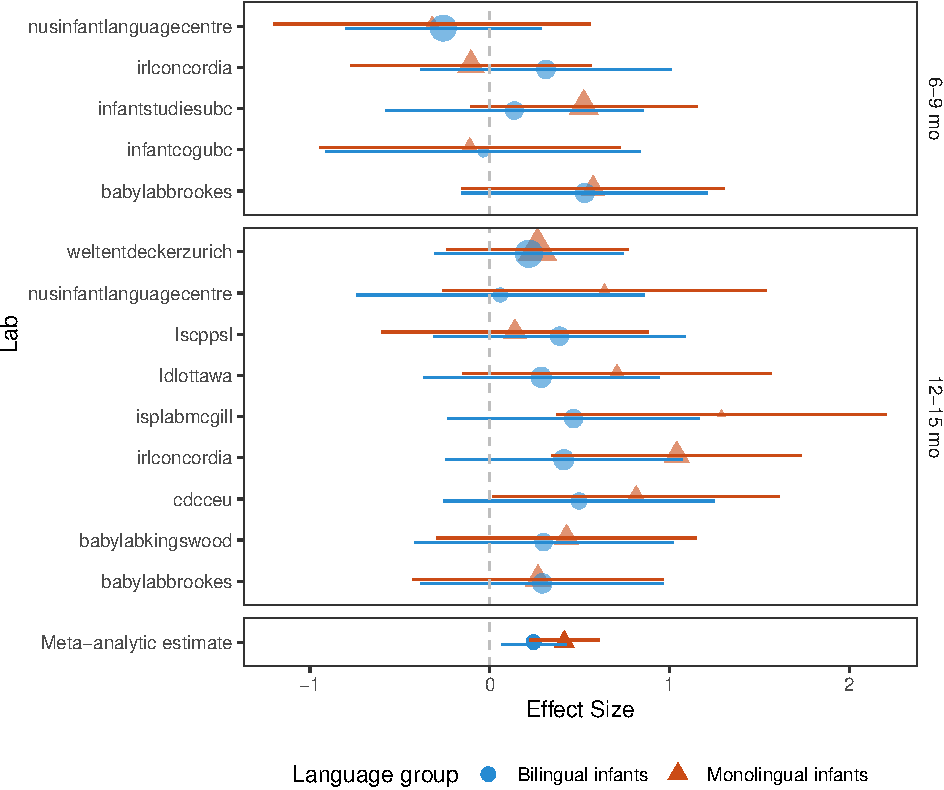
\includegraphics{mb1b-paper_files/figure-latex/unnamed-chunk-3-1.pdf}
\caption{\label{fig:unnamed-chunk-3}Forest plot for the matched dataset. Standardized effect sizes are shown for each lab, with error bars showing 95\% confidence intervals. Each lab reported two effect sizes: one for monolingual group and the other one for bilingual group. Points are scaled by inverse variance and colored by language groups (blue circle denotes bilinguals and red triangle denotes monolinguals). For the age group panels, the point and its associated interval represent the meta-analytic estimate and the 95\% confidence interval in each language group. The points in bottom panel show the global meta-analytic estimate.}
\end{figure}

\hypertarget{within-group-variability-meta-analysis}{%
\paragraph{Within-group variability meta-analysis}\label{within-group-variability-meta-analysis}}

Our second set of pre-registered meta-analyses examined whether the variability in infants' preference for IDS within a sample (within-study variability) was related to language background (monolingual vs.~bilingual). Note that this question of within-sample heterogeneity is different than questions of between-sample heterogeneity that can also be addressed in meta-analysis (see Higgins \& Thompson, 2002; Higgins, Thompson, Deeks, \& Altman, 2003 for approaches to between-group variability in meta-analysis). Specifically, the within-group variability meta-analysis approach provides additional insights of how two groups differ in terms of their variances, not merely their mean effect sizes. This approach is useful when the language backgrounds of the infants influence not only the magnitude of infants' IDS preference, but also the variability of infants' IDS preference. In the following, the standard deviations measure looking time variability of infants' preference for IDS over ADS in each language group (either monolingual or bilingual). Again, we report \(d_z\), an effect size that measures the magnitude of infants' preference for IDS over ADS.

According to Nakagawa et al. (2015), there are two approaches to run within-group variability meta-analysis: one approach uses \(lnCVR\), the natural logarithm of the ratio between the coefficients of variation, to compare the variability of two groups; a second approach enters \(lnSD\) (the natural logarithm of standard deviations) and \(ln\bar{X}\) (the log mean) into a mixed-effect model. The mixed-effect model can be used when the assumption that the standard deviation is proportional to the mean, necessary for the \(lnCVR\) approach, is not met. We found that the standard deviations and effect sizes were not significantly correlated. Therefore, we chose the second, mixed-effect model approach. In the following meta-regression model, the natural logarithm of the standard deviations (lnSD) from each language group is the dependent variable. This dependent variable (group variance) is the log-transformed standard deviation of infants' preference for IDS over ADS that correspond to infants' language group (either monolingual/bilingual).

\[lnSD \sim 1 + bilingual + ln(d_z’) + (bilingual | lab)\]
where \(d_z’\) is the absolute value of \(d_z\) because we needed to ensure that values entered into the logarithm were positive, bilingual is the binary dummy variable that indicates bilingualism - whether the language group is monolingual or bilingual. Further, bilingualism was entered as a random slope in the model.

In the matched dataset, we did not find statistically significant evidence for bilingualism as a moderator of the differences in standard deviations across language groups, (\(d_z\) = -0.08, \(p = .235\)). Similarly, we also did not find statistical significance for bilingualism in the full dataset, (\(d_z\) = 0.03, \(p = .660\)). In short, we did not find support for the hypothesis that bilingual infants would show larger within-group variability than monolingual infants.

\hypertarget{mixed-effects-approach}{%
\subsubsection{Mixed-effects approach}\label{mixed-effects-approach}}

Mixed-effects regression allows variables of interest to be specified on a trial-by-trial and infant-by-infant basis. We had anticipated that we would be able to include additional data from labs that aimed to test homogeneous samples (i.e., because we could include infants from these labs who were not learning this homogeneous language pair), but in practice this did not apply as only one lab contributed a homogeneous data set, and that lab did not test additional infants. We were also able to include data from all valid trials, rather than excluding data from yoked pairs with a missing data point. As under the meta-analytic approach, we ran the models twice, once including only data from labs that contributed matched samples of monolinguals and bilinguals, and once including all available data from 6-9 and 12-15 month-olds.

The mixed-effects model was specified as follows:

\[DV \sim IV_1 + IV_2 + \text{...} + (\text{...} | \text{subject}) + (\text{...} | \text{item}) + (\text{...} | \text{lab})\]

The goal of this framework was to examine effects of the independent variables (IV) on the dependent variable (DV), while controlling for variation in both the DV (\enquote{random intercepts}) and the relationship of the IV to the DV (\enquote{random slopes}) based on relevant grouping units (subjects, items, and labs). Following recent recommendations (Barr, Levy, Scheepers, \& Tily, 2013), we planned to initially fit a maximal random effects structure, such that all random effects appropriate for our design were included in the model. However, we also recognized that such a large random effects structure might be overly complex given our data, and would be unlikely to converge. After reviewer feedback during Stage 1 of the Registered Report review process, we pre-registered a plan to use a \enquote{Parsimonious mixed models} approach for pruning the random effects (Bates et al., 2015a; Matuschek, Kliegl, Vasishth, Baayen, \& Bates, 2017). However, we found that it was computationally difficult to first fit complex models (i.e., our models had multiple interactions and cross-levels grouping) under the maximal random effects structure and then prune the models using a parsimonious mixed models approach. Further, we note that this was not the approach used in MB1, which would make direct comparison between MB1 and the current study difficult. As such, following MB1, we fitted and pruned\footnote{Results reported in this paper were pruned by fitting mixed-effect models with `lme4` version 1.1-21.} the following models using the maximal random effects structure only (Barr et al., 2013). We fit all models using the lme4 package (Bates et al., 2015b) and computed \(p\) values using the lmerTest package (Kuznetsova, Brockhoff, \& Christensen, 2016). Below is a description of our model variables:

\begin{itemize}
\tightlist
\item
  log\_lt: Dependent variable. Log-transformed looking time in seconds.
\item
  trial\_type: A dummy coded variable with two levels, with ADS trials as the baseline, such that positive effects of trial type indicate longer looking to IDS.
\item
  bilingual: A dummy coded variable with two levels, with monolingual as the baseline, such that positive effects of bilingualism reflect longer looking by bilinguals.
\item
  language: A dummy coded variable for whether infants were learning North American English as a native language (i.e., \textgreater{}= 90\% exposure to NAE for monolinguals, or \textgreater{}= 25\% exposure to NAE for bilinguals).
\item
  exp\_nae: A continuous variable for the percent of time infants heard North-American English.
\item
  method: A dummy-coded variable to control for effects of different experimental setups, with single-screen central fixation as the reference level.
\item
  age\_days: Centered for interpretability of main effects.
\item
  trial\_number: The number of the trial pair, recoded such that the first trial pair is 0.
\item
  ses: The number of years of maternal education, centered for ease of interpretation.
\end{itemize}

Note that in this analysis plan, we have used a concise format for model specification, which is the form used in R. As such, lower-order effects subsumed by interactions are modeled even though they are not explicitly written. For example, the interaction trial\_type * trial\_num also assumes a global intercept, a main effect of trial type, and a main effect of trial number.

\hypertarget{homogeneity-of-variance}{%
\paragraph{Homogeneity of variance}\label{homogeneity-of-variance}}

We pre-registered a Levene's test to examine whether monolinguals and bilinguals showed different amounts of variance in their IDS preference. However, we ultimately omitted this test because the null results of our within-group variability meta-analysis did not support a difference between monolingual and bilingual infants in the variance of their IDS preference.

\hypertarget{effects-of-bilingualism-on-ids-preference}{%
\paragraph{Effects of bilingualism on IDS preference}\label{effects-of-bilingualism-on-ids-preference}}

We planned a mixed-effects model which was based on the structure of the final model fit for the ManyBabies monolingual project, including bilingualism as an additional moderator. Note that because data collection for both projects was simultaneous, we did not know prior to registration what the final model structure for the monolingual-only sample would be (it was expected that pruning of this model would be necessary in the case of non-convergence). The original model proposed for the monolingual-only sample was designed to include simple effects of trial type, method, language (infants exposed vs.~not exposed to NAE-IDS), age, and trial number, capturing the basic effects of each parameter on looking time (e.g., longer looking times for IDS, shorter looking times on later trials). Additionally, the model included two-way interactions of trial type with method and with trial number, a two-way interaction of age with trial number, as well as two- and three-way interactions between trial type, age, and language (see ManyBabies Consortium, in press, for full justification). This model was specified to minimize higher-order interactions while preserving theoretically-important interactions. Note that to reduce model complexity, both developmental effects and trial effects are treated linearly. The planned model for ManyBabies monolingual was:

\begin{equation}
\begin{split}
\text{log lt} \sim & \text{trial type} * \text{method} + \text{trial type} * \text{trial num} + \text{age} * \text{trial num} + \\
& \text{trial type} * \text{age} * \text{language} + \\
& (\text{trial type} * \text{trial num} \mid \text{subid}) + \\
& (\text{trial type} * \text{age} \mid \text{lab}) + \\
& (\text{method} + \text{age} * \text{language} \mid \text{item})
\end{split}
\end{equation}

It was expected that pruning would be necessary in the case of non-convergence.

Our analysis plan specified that we would add bilingualism to the fixed effects of the final pruned model that fitted to the monolingual sample. For higher-order interactions in the model, we ensured that we had at least 20 infants per group. For example, for a three-way interaction between bilingualism, language and age, we included at least 20 infants per group: at least 20 infants in the group of 6-9 month-old bilinguals who were not exposed to NAE. We applied the same rules to all other groups.

In our preregistration, we were uncertain as to whether our sample size would support a model with a four-way-interaction of trial type, age, bilingual status, and language. Given our final sample size, we elected to fit our main model without including the four-way interaction effect\footnote{We did not enter the above-mentioned four-way interaction into our main model, but note that in the more complex model, the four-way interaction was not statistically significant in the matched dataset ($\beta$ = 0.00, $SE = 0.02$, $p = 0.85$) or the full dataset ($\beta$ = 0.01, $SE = 0.01$, $p = 0.63$).}. In our main model, we included two fixed three-way interactions: (i) the interaction between bilingualism, age and trial type, and (ii) the interaction between language, age and trial type, as well as other subsumed lower-order interactions.

Regardless of our fixed effect structure, the model included the random slope of bilingualism on lab and item, as well as appropriate interactions with other random factors. Our initial unpruned model was:

\begin{equation}
\begin{split}
\text{log lt} \sim & \text{trial type} * \text{method} + \text{trial type} * \text{trial num} + \text{age} * \text{trial num} + \\
& \text{trial type} * \text{age} * \text{language} + \\
& \text{trial type} * \text{age} * \text{bilingual} + \\
& (\text{trial type} * \text{trial num} \mid \text{subid}) + \\
& (\text{trial type} * \text{age} * \text{bilingual} \mid \text{lab}) + \\
& (\text{method} + \text{age} * \text{language} + \text{age} * \text{bilingual} \mid \text{item})
\end{split}
\end{equation}

After pruning random effects for non-convergence and singularity, the final models for the matched dataset and full dataset were different. The following was the final model of the matched dataset:

\begin{equation}
\begin{split}
\text{log lt} \sim & \text{trial type} * \text{method} + \text{trial type} * \text{trial num} + \text{age} * \text{trial num} + \\
& \text{trial type} * \text{age} * \text{language} + \\
& \text{trial type} * \text{age} * \text{bilingual} + \\
& (1 \mid \text{subid}) + \\
& (\text{bilingual} \mid \text{lab}) + \\
& (1 \mid \text{item})
\end{split}
\end{equation}

In contrast, the final model of the full dataset was:

\begin{equation}
\begin{split}
\text{log lt} \sim & \text{trial type} * \text{method} + \text{trial type} * \text{trial num} + \text{age} * \text{trial num} + \\
& \text{trial type} * \text{age} * \text{language} + \\
& \text{trial type} * \text{age} * \text{bilingual} + \\
& (1 \mid \text{subid}) + \\
& (1 \mid \text{lab}) + \\
& (1 \mid \text{item})
\end{split}
\end{equation}

\begin{table}[tbp]

\begin{center}
\begin{threeparttable}

\caption{\label{tab:unnamed-chunk-8}Linear Mixed Model 1 testing bilingualism effect on IDS in a matched dataset.}

\begin{tabular}{lllll}
\toprule
 & \multicolumn{1}{c}{Estimate} & \multicolumn{1}{c}{SE} & \multicolumn{1}{c}{t} & \multicolumn{1}{c}{p}\\
\midrule
Intercept & 1.930 & 0.074 & 26.000 & 0.000\\
IDS & 0.093 & 0.047 & 2.000 & 0.050\\
HPP & 0.103 & 0.092 & 1.110 & 0.283\\
Single Screen & 0.113 & 0.103 & 1.090 & 0.288\\
Age & -0.027 & 0.008 & -3.410 & 0.001\\
Trial \# & -0.036 & 0.003 & -13.900 & 0.000\\
NAE & -0.059 & 0.075 & -0.792 & 0.435\\
Bilingual & 0.000 & 0.034 & 0.008 & 0.994\\
IDS * HPP & 0.016 & 0.029 & 0.566 & 0.571\\
IDS * Single Screen & 0.004 & 0.031 & 0.124 & 0.901\\
Age * Trial \# & 0.001 & 0.000 & 2.270 & 0.023\\
IDS * Trial \# & 0.001 & 0.004 & 0.175 & 0.862\\
IDS * Age & 0.013 & 0.006 & 2.180 & 0.029\\
IDS * NAE & 0.051 & 0.026 & 1.950 & 0.052\\
Age * NAE & 0.007 & 0.010 & 0.646 & 0.519\\
IDS * Bilingual & -0.012 & 0.024 & -0.522 & 0.602\\
Age * Bilingual & -0.006 & 0.009 & -0.671 & 0.503\\
IDS * Age * NAE & 0.016 & 0.008 & 1.860 & 0.063\\
IDS * Age * Bilingual & -0.009 & 0.008 & -1.210 & 0.227\\
\bottomrule
\end{tabular}

\end{threeparttable}
\end{center}

\end{table}

\begin{table}[tbp]

\begin{center}
\begin{threeparttable}

\caption{\label{tab:unnamed-chunk-8}Linear Mixed Model 1 testing bilingualism effect on IDS in a full dataset.}

\begin{tabular}{lllll}
\toprule
 & \multicolumn{1}{c}{Estimate} & \multicolumn{1}{c}{SE} & \multicolumn{1}{c}{t} & \multicolumn{1}{c}{p}\\
\midrule
Intercept & 1.890 & 0.047 & 40.400 & 0.000\\
IDS & 0.106 & 0.038 & 2.770 & 0.009\\
HPP & 0.190 & 0.058 & 3.310 & 0.002\\
Single Screen & 0.243 & 0.054 & 4.510 & 0.000\\
Age & -0.029 & 0.005 & -5.680 & 0.000\\
Trial \# & -0.037 & 0.002 & -21.200 & 0.000\\
NAE & 0.003 & 0.048 & 0.063 & 0.950\\
Bilingual & -0.006 & 0.025 & -0.234 & 0.815\\
IDS * HPP & 0.029 & 0.018 & 1.620 & 0.106\\
IDS * Single Screen & -0.020 & 0.019 & -1.060 & 0.291\\
Age * Trial \# & 0.001 & 0.000 & 3.910 & 0.000\\
IDS * Trial \# & -0.002 & 0.002 & -0.961 & 0.337\\
IDS * Age & 0.013 & 0.003 & 3.800 & 0.000\\
IDS * NAE & 0.038 & 0.016 & 2.420 & 0.015\\
Age * NAE & 0.002 & 0.007 & 0.244 & 0.807\\
IDS * Bilingual & 0.003 & 0.019 & 0.142 & 0.887\\
Age * Bilingual & -0.003 & 0.008 & -0.369 & 0.712\\
IDS * Age * NAE & 0.009 & 0.005 & 1.960 & 0.051\\
IDS * Age * Bilingual & -0.007 & 0.006 & -1.110 & 0.265\\
\bottomrule
\end{tabular}

\end{threeparttable}
\end{center}

\end{table}

Overall, the mixed-level analyses in both matched and full datasets yielded similar results (Table 2 and 3). More coefficients were statistically significant in the full dataset, likely due to the larger sample size. Thus, in the following, we focus on the results of the mixed-level model for the full dataset. We found that infants showed a preference for IDS, as indicated by a positive coefficient on the IDS predictor (reflecting greater looking times to IDS stimuli). We did not find any effects of the bilingualism on IDS preference nor any interaction effects between bilingualism and other moderators. This finding is consistent with the results of our meta-analysis above.

Surprisingly, the fitted model did not show an interaction between infants' IDS preference and the method used in the lab, a result that is different from the results in the MB1 project. However, this finding is likely due to smaller sample sizes in the current paper, as we restricted the analysis to participants at particular ages. Apart from this, our findings were largely consistent with the MB1 study. There was a significant and positive two-way interaction between IDS and NAE, suggesting greater IDS preferences for children in NAE contexts. The interaction between IDS and age was also significant and positive, suggesting that older children showed a stronger IDS preference. Finally, we found a marginally significant three-way interaction between IDS, age, and NAE, suggesting that older children in NAE contexts tended to show stronger IDS preference than those in the non-NAE contexts.

\hypertarget{dose-effects-of-exposure-to-nae-ids-in-bilingual-infants}{%
\paragraph{Dose effects of exposure to NAE-IDS in bilingual infants}\label{dose-effects-of-exposure-to-nae-ids-in-bilingual-infants}}

In this analysis, we tested whether we could observe a dose-response relationship between infants' exposure to NAE-IDS (measured continuously) and their preference for IDS over ADS.

We decided to conduct this analysis only including data from bilinguals. Our reasoning was that bilingualism status and exposure to NAE-IDS are confounded, as monolinguals' exposure to NAE will be either near 0\% or 100\%, while bilinguals' NAE experience can be either 0\%, or 25-75\%. Because the monolingual sample is larger and their NAE exposures are more extreme, their effects would dominate that of the bilinguals in a merged analysis. Therefore, we reasoned that if there is a dose effect, it should be observable in the bilingual sample alone. Finally, although excluding monolingual infants reduced power overall, we decided that given the relatively large sample of bilingual infants, this disadvantage would be offset by the ease of interpretation afforded by restricting the analysis to bilinguals.

Once again, we based this model on the final pruned monolingual model, substituting the binary measure of exposure to NAE-IDS (language) with the continuous measure of exposure(exp\_nae), and including a random slope for exp\_nae by item (which was ultimately pruned from the model). After pruning, our model was specified as follows:

\begin{equation}
\begin{split}
\text{log lt} \sim & \text{trial type} * \text{method} + \text{trial type} * \text{trial num} + \text{age} * \text{trial num} + \\
& \text{trial type} * \text{age} * \text{exp nae} + \\
& (1\mid \text{subid}) + \\
& (\text{trial type} \mid \text{lab}) + \\
& (1 \mid \text{item})
\end{split}
\end{equation}

\begin{table}[tbp]

\begin{center}
\begin{threeparttable}

\caption{\label{tab:unnamed-chunk-9}Linear Mixed Model testing the effects of exposure to NAE-IDS in bilingual infants.}

\begin{tabular}{lllll}
\toprule
 & \multicolumn{1}{c}{Estimate} & \multicolumn{1}{c}{SE} & \multicolumn{1}{c}{t} & \multicolumn{1}{c}{p}\\
\midrule
Intercept & 1.910 & 0.074 & 25.900 & 0.000\\
IDS & -0.009 & 0.062 & -0.138 & 0.891\\
HPP & 0.088 & 0.091 & 0.963 & 0.354\\
Single Screen & 0.168 & 0.111 & 1.510 & 0.160\\
Age & -0.024 & 0.010 & -2.270 & 0.024\\
Trial \# & -0.036 & 0.004 & -10.100 & 0.000\\
EXP\_NAE & -0.001 & 0.001 & -0.565 & 0.575\\
IDS * HPP & 0.054 & 0.053 & 1.020 & 0.331\\
IDS * Single Screen & 0.028 & 0.060 & 0.465 & 0.654\\
Age * Trial \# & 0.000 & 0.001 & 0.300 & 0.764\\
IDS * Trial \# & 0.006 & 0.005 & 1.150 & 0.251\\
IDS * Age & 0.006 & 0.008 & 0.781 & 0.435\\
IDS * EXP\_NAE & 0.002 & 0.001 & 2.860 & 0.011\\
Age * EXP\_NAE & 0.000 & 0.000 & -0.200 & 0.842\\
IDS * Age * EXP\_NAE & 0.000 & 0.000 & 0.891 & 0.373\\
\bottomrule
\end{tabular}

\end{threeparttable}
\end{center}

\end{table}

Table 4 contains the details of the results in this model. The main effect of infants' exposure to NAE (exp\_nae) was not significant (\(\beta\) = , \$SE = \$, \(p = )\). This indicates that bilingual infants who were exposed to more NAE did not pay more attention to the NAE speech stimuli than those who were exposed to less NAE. However, the interaction between trial type and exp\_nae was significant (\(\beta\) = , \$SE = \$, \(p = )\). That is, bilingual infants who were exposed to more NAE showed stronger IDS preferences, confirming a dose-response relationship between infants' exposure to NAE and their preference for IDS over ADS (Figure 2) even among bilinguals who are learning NAE as one of their native languages.

\begin{figure}
\centering
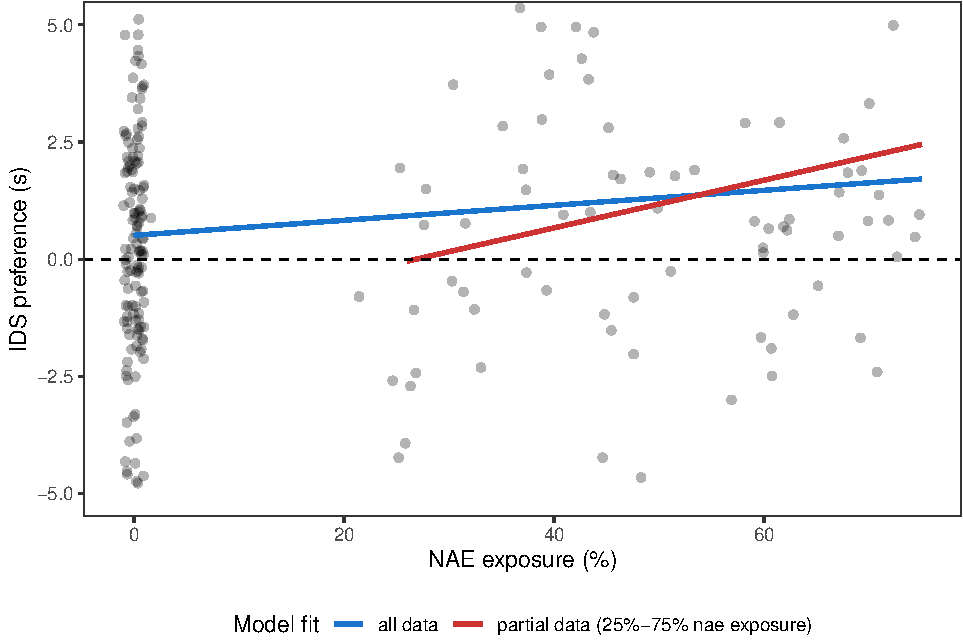
\includegraphics{mb1b-paper_files/figure-latex/fig2-1.pdf}
\caption{\label{fig:fig2}Linear trend between infants' IDS preference and their percentage of time exposed to NAE. Blue line indicates a regression model between infants' IDS preference and their NAE exposure (starting from zero). Red line indicates another regression model of the same relationship with a focus of NAE exposure between 25 to 75\%. Finally, we note that the y-axis was truncated to highlight the trend such that some individual points are not plotted.}
\end{figure}

\hypertarget{socio-economic-status-as-a-moderator-of-monolingual-bilingual-differences}{%
\paragraph{Socio-economic status as a moderator of monolingual-bilingual differences}\label{socio-economic-status-as-a-moderator-of-monolingual-bilingual-differences}}

Because socio-economic status can vary systematically between monolinguals and bilinguals in the same community, we were interested in whether relationships between bilingualism and IDS preference would hold when controlling for socio-economic status. It is possible that an observed effect of bilingualism on IDS preference could disappear once SES was controlled. Alternatively, it is possible that the effect of bilingualism on IDS preference could only be apparent once SES was controlled. Thus, this analysis was important regardless of an observed relationship between IDS preference and bilingualism in the previous model.

Our approach was to add SES as a moderator of our final model for bilinguals. We expected that any effects of socio-economic status could interact with age, thus this model included interactions of trial type, age, and socio-economic status as a fixed effect, as well as the corresponding random slope by item. Based on the potential model detailed above for the bilinguals, our expected ses-mediated model was:

\begin{equation}
\begin{split}
\text{log lt} \sim & \text{trial type} * \text{method} + \text{trial type} * \text{trial num} + \text{age} * \text{trial num} + \\
& \text{trial type} * \text{age} * \text{language} + \\
& \text{trial type} * \text{age} * \text{bilingual} + \\
& \text{trial type} * \text{age} * \text{ses} + \\
& (\text{trial type} * \text{trial num} \mid \text{subid}) + \\
& (\text{trial type} * \text{age} * \text{bilingual} \mid \text{lab}) + \\
& (\text{method} + \text{age} * \text{language} + \text{age} * \text{bilingual} +
\text{age} * \text{ses} \mid \text{item})
\end{split}
\end{equation}

After pruning for non-convergence, our final model specifications are listed below. For the matched dataset, the final model was:

\begin{equation}
\begin{split}
\text{log lt} \sim & \text{trial type} * \text{method} + \text{trial type} * \text{trial num} + \text{age} * \text{trial num} + \\
& \text{trial type} * \text{age} * \text{language} + \\
& \text{trial type} * \text{age} * \text{bilingual} + \\
& \text{trial type} * \text{age} * \text{ses} + \\
& (1 \mid \text{subid}) + \\
& (\text{bilingual} \mid \text{lab}) 
\end{split}
\end{equation}

By contrast, the final model of the full dataset was:

\begin{equation}
\begin{split}
\text{log lt} \sim & \text{trial type} * \text{method} + \text{trial type} * \text{trial num} + \text{age} * \text{trial num} + \\
& \text{trial type} * \text{age} * \text{language} + \\
& \text{trial type} * \text{age} * \text{bilingual} + \\
& \text{trial type} * \text{age} * \text{ses} + \\
& (1 \mid \text{subid}) + \\
& (1 \mid \text{lab}) + \\
& (1 \mid \text{item})
\end{split}
\end{equation}

\begin{table}[tbp]

\begin{center}
\begin{threeparttable}

\caption{\label{tab:unnamed-chunk-11}Linear Mixed Model 3 examining socio-economic status as a moderator of monolingual-bilingual differences SES in the matached dataset.}

\begin{tabular}{lllll}
\toprule
 & \multicolumn{1}{c}{Estimate} & \multicolumn{1}{c}{SE} & \multicolumn{1}{c}{t} & \multicolumn{1}{c}{p}\\
\midrule
Intercept & 1.960 & 0.108 & 18.200 & 0.000\\
IDS & 0.075 & 0.080 & 0.936 & 0.349\\
HPP & 0.120 & 0.089 & 1.340 & 0.199\\
Single Screen & 0.094 & 0.100 & 0.939 & 0.359\\
Age & -0.025 & 0.029 & -0.881 & 0.378\\
Trial \# & -0.033 & 0.002 & -17.200 & 0.000\\
NAE & -0.089 & 0.072 & -1.240 & 0.225\\
Bilingual & 0.022 & 0.028 & 0.795 & 0.427\\
SES & -0.003 & 0.005 & -0.513 & 0.608\\
IDS * HPP & 0.019 & 0.030 & 0.633 & 0.527\\
IDS * Single Screen & 0.006 & 0.032 & 0.201 & 0.841\\
Age * Trial \# & 0.001 & 0.000 & 2.330 & 0.020\\
IDS * Trial \# & -0.005 & 0.003 & -1.740 & 0.081\\
IDS * Age & 0.070 & 0.025 & 2.770 & 0.006\\
IDS * NAE & 0.054 & 0.028 & 1.960 & 0.050\\
Age * NAE & 0.012 & 0.010 & 1.130 & 0.260\\
IDS * Bilingual & -0.018 & 0.025 & -0.734 & 0.463\\
Age * Bilingual & -0.010 & 0.009 & -1.160 & 0.246\\
IDS * SES & 0.003 & 0.005 & 0.770 & 0.441\\
Age * SES & 0.000 & 0.002 & -0.147 & 0.883\\
IDS * Age * NAE & 0.016 & 0.009 & 1.810 & 0.071\\
IDS * Age * Bilingual & -0.005 & 0.008 & -0.606 & 0.545\\
IDS * Age * SES & -0.004 & 0.002 & -2.330 & 0.020\\
\bottomrule
\end{tabular}

\end{threeparttable}
\end{center}

\end{table}

\begin{table}[tbp]

\begin{center}
\begin{threeparttable}

\caption{\label{tab:unnamed-chunk-11}Linear Mixed Model 3 examining socio-economic status as a moderator of monolingual-bilingual differences SES in the full dataset.}

\begin{tabular}{lllll}
\toprule
 & \multicolumn{1}{c}{Estimate} & \multicolumn{1}{c}{SE} & \multicolumn{1}{c}{t} & \multicolumn{1}{c}{p}\\
\midrule
Intercept & 1.940 & 0.080 & 24.200 & 0.000\\
IDS & 0.051 & 0.066 & 0.781 & 0.436\\
HPP & 0.189 & 0.063 & 2.990 & 0.004\\
Single Screen & 0.202 & 0.064 & 3.170 & 0.003\\
Age & -0.021 & 0.020 & -1.050 & 0.292\\
Trial \# & -0.037 & 0.002 & -19.500 & 0.000\\
NAE & -0.018 & 0.051 & -0.363 & 0.718\\
Bilingual & 0.003 & 0.026 & 0.109 & 0.913\\
SES & -0.001 & 0.004 & -0.204 & 0.838\\
IDS * HPP & 0.029 & 0.020 & 1.410 & 0.160\\
IDS * Single Screen & -0.022 & 0.021 & -1.040 & 0.296\\
Age * Trial \# & 0.001 & 0.000 & 4.280 & 0.000\\
IDS * Trial \# & -0.003 & 0.003 & -0.949 & 0.343\\
IDS * Age & 0.021 & 0.017 & 1.250 & 0.213\\
IDS * NAE & 0.031 & 0.017 & 1.800 & 0.072\\
Age * NAE & 0.003 & 0.007 & 0.443 & 0.657\\
IDS * Bilingual & -0.007 & 0.020 & -0.336 & 0.737\\
Age * Bilingual & -0.002 & 0.008 & -0.206 & 0.837\\
IDS * SES & 0.004 & 0.003 & 1.220 & 0.222\\
Age * SES & -0.001 & 0.001 & -0.781 & 0.435\\
IDS * Age * NAE & 0.012 & 0.005 & 2.230 & 0.026\\
IDS * Age * Bilingual & -0.004 & 0.007 & -0.597 & 0.550\\
IDS * Age * SES & -0.001 & 0.001 & -0.599 & 0.549\\
\bottomrule
\end{tabular}

\end{threeparttable}
\end{center}

\end{table}

In general, across the matched and full datasets (Table 5 and 6), SES did not have a significant effect on infants' looking time nor did it affect infants' preference for IDS. However, for the matched dataset only, we found a statistically significant three-way interaction between IDS, age, and SES. Specifically, infants from 6- to 9-month-olds showed stronger IDS preference when they were from a higher SES families, but older infants from 12- to 15-month-olds showed similar IDS preference across families with different SES levels. However, this interaction was not observed in the full dataset, raising the possibility that it is a spurious, and arose only in the matched dataset because it is substantially smaller than the full data set.

\hypertarget{exploratory-analyses}{%
\subsection{Exploratory analyses}\label{exploratory-analyses}}

\hypertarget{the-relationship-between-nae-and-ids-for-bilingual-infants-who-have-some-exposure-to-nae}{%
\subsubsection{The relationship between NAE and IDS for bilingual infants who have some exposure to NAE}\label{the-relationship-between-nae-and-ids-for-bilingual-infants-who-have-some-exposure-to-nae}}

In our second confirmatory analysis model (linear mixed model 2), we found that bilingual infants with more exposure to NAE showed stronger IDS preference. However, this initial analysis included a number of bilingual infants who were not exposed to NAE at all (Figure 2). This raises the question of whether the relation between NAE and IDS preference may be primarily driven by the infants who were not learning NAE. In the following analysis, we re-ran the pre-registered NAE-IDS model by restricting the model to infants who were exposed to NAE between 25\% and 75\% of the time. After pruning for non-convergence, the final model was:

\begin{equation}
\begin{split}
\text{log lt} \sim & \text{trial type} * \text{method} + \text{trial type} * \text{trial num} + \text{age} * \text{trial num} + \\
& \text{trial type} * \text{age} * \text{exp nae} + \\
& (1 \mid \text{subid}) + \\
& (1 \mid \text{lab}) + \\
& (1 \mid \text{item})
\end{split}
\end{equation}

\begin{table}[tbp]

\begin{center}
\begin{threeparttable}

\caption{\label{tab:unnamed-chunk-13}Linear Mixed Model testing the effects of exposure to NAE-IDS (restricted to bilingual infants living in NAE contexts).}

\begin{tabular}{lllll}
\toprule
 & \multicolumn{1}{c}{Estimate} & \multicolumn{1}{c}{SE} & \multicolumn{1}{c}{t} & \multicolumn{1}{c}{p}\\
\midrule
Intercept & 1.910 & 0.168 & 11.400 & 0.000\\
IDS & -0.211 & 0.132 & -1.600 & 0.112\\
HPP & 0.227 & 0.142 & 1.600 & 0.180\\
Single Screen & 0.094 & 0.200 & 0.472 & 0.663\\
Age & -0.009 & 0.036 & -0.265 & 0.791\\
Trial \# & -0.041 & 0.006 & -7.410 & 0.000\\
EXP\_NAE & -0.002 & 0.002 & -0.783 & 0.434\\
IDS * HPP & 0.016 & 0.063 & 0.260 & 0.795\\
IDS * Single Screen & -0.115 & 0.081 & -1.420 & 0.156\\
Age * Trial \# & 0.001 & 0.001 & 1.230 & 0.219\\
IDS * Trial \# & 0.016 & 0.008 & 1.990 & 0.048\\
IDS * Age & 0.022 & 0.030 & 0.720 & 0.472\\
IDS * EXP\_NAE & 0.005 & 0.002 & 2.900 & 0.004\\
Age * EXP\_NAE & 0.000 & 0.001 & -0.653 & 0.515\\
IDS * Age * EXP\_NAE & 0.000 & 0.001 & 0.054 & 0.957\\
\bottomrule
\end{tabular}

\end{threeparttable}
\end{center}

\end{table}

Based on 135 infants, the interaction between Trial Type and NAE exposure was still statistically significant (\(\beta\) = , \$SE = \$, \(p = )\). This result suggested that a dose-response relationship between infants' exposure to NAE and their preference for IDS over ADS was not driven by infants living in non-NAE contexts alone (see Table 7 for details of the model).

\hypertarget{general-discussion}{%
\section{General Discussion}\label{general-discussion}}

The current study was designed to better understand the effects of experience on the tuning of infants' preference for infant-directed speech (IDS) compared to adult-directed speech (ADS). Bilingual infants' language experience is split across input in two different languages, which are being acquired simultaneously. Bilinguals and monolinguals may thus differ in their preference for IDS. To explore this question, we used a collaborative, multi-lab (N = 17 labs) approach to gather a large dataset of infants who were either 6-9- or 12-15-months old and growing up bilingual (N = 333 bilingual infants in the final sample, and a lab-matched sample of N = 385 monolingual infants from the same communities). Data were collected as a companion project to ManyBabies 1 (ManyBabies Consortium, in press), which was limited to infants growing up monolingual. Overall, we found that bilingualism neither enhanced nor attenuated infants' preference for IDS, with bilinguals showing a similar magnitude and developmental trajectory of IDS preference as monolinguals from age 6 to 15 months.

Although bilingual experience did not appear to moderate infants' preference for IDS, we found striking evidence that experience hearing North-American English (NAE, the language of our stimuli) contributed to the magnitude of bilingual infants' IDS preference. Bilinguals with greater exposure to NAE showed greater IDS preferences (when tested in NAE) than those who had less exposure to NAE. This relationship between NAE exposure and IDS preference was also observed in a subsample of bilingual infants all acquiring NAE, but who varied in how much they were exposed to NAE relative to their other native language. These results converge with those from the larger ManyBabies 1 monolingual study, which reported that monolinguals acquiring NAE had a stronger preference for IDS than monolinguals acquiring another language. Importantly, our approach provides a more nuanced view of the relationship between NAE and IDS preference, and suggests that there is a continuous dose effect of exposure on preference. Together, our findings have a number of implications for bilingual language acquisition during infancy. In the following, we will first discuss each of our research questions in turn, followed by limitations and implications of our study.

Our first research question asked whether bilingualism affects infants' attention to IDS relative to ADS. We hypothesized that the complexity of the bilingual infant's learning experience might lead to greater reliance on/preference for IDS, given that IDS may be viewed as an enhanced linguistic signal. However, this hypothesis was not confirmed. We observed a meta-analytic effect size in the full dataset for monolinguals of \(d_z\) =
0.36 {[}CI = 0.28 - 0.44{]} and for bilinguals of \(d_z\) = 0.26 {[}CI: 0.09 - 0.43{]}. While monolinguals showed a numerically larger effect size, this difference was not statistically significant in either the meta-analyses or the mixed-effects linear models. Although small differences are still possible, our data generally support the conclusion that bilingual and monolingual infants show a similar preference for IDS over ADS. Specifically, both groups show a preference for IDS at 6-9 months of age, which gets stronger by 12-15 months.

An additional part of our first research question asked whether bilinguals might show more variability than monolinguals in their IDS preference, beyond any differences in the magnitude of the preference. We had reasoned that given their diversity of language experiences, bilingual groups may have a higher heterogeneity in terms of their IDS preference compared to monolingual groups (see also Orena \& Polka, 2019, for a recent experiment that observed this pattern). However, while both monolingual and bilingual groups showed high variability, there were no reliable differences in variability observed across groups. Thus, our results did not support the idea that bilingual infants show more variable IDS preference than their monolingual peers.

Given that monolinguals and bilinguals can systematically differ in their socio-economic status (SES), the third part of our first research question asked whether SES might moderate bilingualism effects. We found mixed support for the role of SES in our datasets. In our smaller dataset (matched dataset across labs), we found a statistically significant interaction between age, SES, and IDS preference: 6-9-month-olds from higher SES families showed stronger IDS preference than those from lower SES families, whereas 12-15-month-olds showed similar IDS preference regardless of SES. The direction of this effect aligns with other research reporting that children from higher SES families generally receive more language input and/or higher quality input (e.g., engaging in conversations with more lexical diversity, complexity, and structural variations) than children from lower SES families (Fernald, Marchman, \& Weisleder, 2013; Hart \& Risley, 1995; Hoff, 2006; Tal \& Arnon, 2018). Thus, this could suggest that infants from higher SES families may show stronger IDS preference earlier in life as they hear more or higher quality IDS in their daily lives. Further, this positive SES impact may be most beneficial to younger infants whose IDS preference is still developing. However, given that in our larger (full) dataset SES was unrelated to IDS preference in either 6-9- or 12-15-month-olds, this result might be spurious and should be interpreted with caution.

Our second research question asked whether and how the amount of exposure to NAE would affect bilingual infants' listening preferences. Given that our stimuli were produced in NAE, we expected that greater exposure to NAE would be linked to greater attention to NAE IDS relative to NAE ADS. Indeed, ManyBabies 1 (ManyBabies Consortium, in press), which was conducted concurrently with the current study, found that that monolinguals acquiring NAE showed a stronger IDS preference than monolinguals not acquiring NAE. However, in the ManyBabies 1 study, exposure to NAE-IDS was a binary variable -- either the infants heard only NAE or heard only a different language in their language environments. In the current paper, bilinguals provide a more nuanced way to address this question, as bilinguals' exposure to NAE varied continuously between 25\% and 75\% (for infants learning NAE as one of their native languages) or was near 0\% (for infants learning two non-NAE native languages). We found clear evidence for a positive dose-response relationship between exposure to NAE and infants' preference for NAE-IDS. This evidence -- that bilinguals with more exposure to NAE showed a stronger NAE-IDS preference -- was also present when focusing only on bilinguals who were learning NAE as one of their native languages (i.e., those exposed to NAE 25-75\% of the time). Importantly, we did not find a similar effect of exposure to NAE on infants' overall looking. This suggests that the effect of NAE exposure on preference for IDS is a meaningful relationship, rather than an artefact due to the stimuli being presented in NAE. Further studies with stimuli in other languages would be necessary to solidify this conclusion.

As the first study to recruit and test bilingual infants at such a large scale and at so many sites, we encountered several challenges (see also Byers-Heinlein et al., under review, for a fuller discussion of challenges in planning and conducting ManyBabies 1). First, several laboratories were not able to recruit the number of bilingual infants they had originally planned. All labs committed to collecting a minimum of 16 bilingual infants per age group. This ended up being unfeasible for some labs within the timeframe available (which was more than a year), in some cases due to a high number of participants not meeting our strict criterion for inclusion as bilingual. This undoubtedly highlights the challenges for labs in recruiting bilingual infant samples, and moreover raises questions about how bilingualism should be defined, and whether it should be treated as a continuous vs.~categorical variable (Anderson, Mak, \& Bialystok, 2018; Bialystok, Luk, Peets, \& Yang, 2018; Incera \& McLennan, 2018). Second, we had planned to explore the effect of different language pairs on IDS preference. We had expected that some labs would be able to recruit relatively homogeneous samples of infants (i.e., all learning the same language pair), but in the end only one of 17 labs did so (another lab had planned to recruit a homogeneous sample but deviated from this plan when it appeared unfeasible). Thus, we leave the question of the effect of language pair on infants' IDS preference an open issue to be followed up in future studies. By and large, we believe that our large-scale approach to data collection may in the future allow for the creation of homogeneous samples of infants tested at different laboratories around the world. As such, large-scale and multi-site bilingual research projects provide researchers with a powerful way to examine how the diversity and variability of bilinguals impact their language and cognitive development.

Overall, our finding that bilinguals show similar preference for IDS as monolinguals reinforces theoretical views that emphasize the similarities in attentional and learning mechanisms across monolingual and bilingual infants (e.g., Curtin, Byers-Heinlein, \& Werker, 2011). IDS appears to be a signal that enhances attention in infants from a variety of language backgrounds. Yet, bilingual infants appear to be exquisitely fine-tuned to the relative amount of input in each of their languages. It could have been the case that language exposure has a threshold effect with any regular exposure to NAE enhancing infants' preference for NAE-IDS, marking it is a highly relevant speech signal. Instead, we observed a graded effect such that the magnitude of bilingual infants' preference varied continuously with the amount of exposure to NAE. Just as bilingual infants' relative vocabulary size and early grammar skills in each language are linked to the amount of input in that language (Hoff et al., 2012; Place \& Hoff, 2011), the current study shows that the amount of language input may also play an important role in other language acquisition processes. Indeed, an intriguing but untested possibility is that different input-related attentional biases (i.e., IDS preference) across bilinguals' two languages explain important variability in the early development of bilingual children's vocabulary and grammar. Future bilingual work can investigate the above possibility to further delineate the interplay between infants' language input, IDS preference, vocabulary, and grammar skills.

To conclude, the findings of the current study provide a more nuanced view of the development of infants' preference for IDS than prior studies have allowed. IDS preference develops along a similar trajectory across infants from monolingual and bilingual backgrounds. Importantly, by testing bilingual infants, our results revealed that this IDS preference operates in a dose-response fashion, where the amount of exposure to NAE positively moderated infants' (NAE-) IDS preference in a continuous way. Our experience highlights the challenges in recruiting and testing bilingual infants, but also reveals the promise of large-scale collaborations for increasing sample sizes, and thus improving the replicability and generalizability of key findings in infant research.

\hypertarget{author-contributions}{%
\section{Author Contributions}\label{author-contributions}}

Author contribution initials reflect authorship order. KBH, MCF, JG, MS contributed to the study concept. KBH, MCF, JG, KK, CLW, MM, MS contributed to the study design. KBH, CB contributed to the final protocol. KBH contributed to study documentation. KBH contributed to study management. KBH, ASMT, AB, AB, SD, CTF, ACF, AG, JG, NGG, JKH, NH, MH, SK, KK, CLW, LL, CM, MM, VM, CN, AJO, LP, CEP, LS, MS, MS, CW, JW contributed to data collection. KBH, ASMT, CB, MCF, JK contributed to data analysis. KBH, CB, AB, MJC, CTF, MCF, JG, NGG, JKH, CLW, LS, MS contributed to the stage 1 manuscript. KBH, ASMT, CTF, MCF, JG, LS, MS contributed to the stage 2 manuscript.

\hypertarget{conflicts-of-interest}{%
\section{Conflicts of Interest}\label{conflicts-of-interest}}

The authors declare that there were no conflicts of interest with respect to the authorship or the publication of this article.

\hypertarget{preregistration}{%
\subsection{Preregistration}\label{preregistration}}

Our manuscript was reviewed prior to data collection (\url{https://osf.io/wtfuq/files/}); in addition, we registered our instructions and materials prior to data collection (\url{https://osf.io/zauhq/}).

\hypertarget{data-materials-and-online-resources}{%
\subsection{Data, materials, and online resources}\label{data-materials-and-online-resources}}

All data and analytic code are available at \url{https://github.com/manybabies/mb1b-analysis-public}. All materials are available via the ManyBabies 1 monolingual Open Science Framework site at osf.io/re95x/.

\newpage

\hypertarget{references}{%
\section{References}\label{references}}

\begingroup
\setlength{\parindent}{-0.5in}
\setlength{\leftskip}{0.5in}

\hypertarget{refs}{}
\leavevmode\hypertarget{ref-anderson_2018}{}%
Anderson, J., Mak, A., L.and Keyvani Chahi, \& Bialystok, E. (2018). The language and social background questionnaire: Assessing degree of bilingualism in a diverse population. \emph{Behavior Research Methods}, \emph{50}(1), 250--263. \url{https://doi.org/10.3758/s13428-017-0867-9}

\leavevmode\hypertarget{ref-barr_2013}{}%
Barr, D. J., Levy, R., Scheepers, C., \& Tily, H. J. (2013). Random effects structure for confirmatory hypothesis testing: Keep it maximal. \emph{Journal of Memory and Language}, \emph{68}(3), 255--278. \url{https://doi.org/https://doi.org/10.1016/j.jml.2012.11.001}

\leavevmode\hypertarget{ref-bates_2015a}{}%
Bates, D., Kliegl, R., Vasishth, S., \& Baayen, H. (2015a). \emph{Parsimonious mixed models}. Preprint.

\leavevmode\hypertarget{ref-bates_2015b}{}%
Bates, D., Mächler, M., Bolker, B., \& Walker, S. (2015b). Fitting linear mixed-effects models using lme4. \emph{Journal of Statistical Software, Articles}, \emph{67}(1), 1--48. \url{https://doi.org/10.18637/jss.v067.i01}

\leavevmode\hypertarget{ref-bialystok_2005}{}%
Bialystok, E., Luk, G., \& Kwan, E. (2005). Bilingualism, biliteracy, and learning to read: Interactions among languages and writing systems. \emph{Scientific Studies of Reading}, \emph{9}(1), 43--61. \url{https://doi.org/10.1207/s1532799xssr0901_4}

\leavevmode\hypertarget{ref-bialystok_2018}{}%
Bialystok, E., Luk, G., Peets, K. F., \& Yang, S. (2018). Receptive vocabulary differences in monolingual and bilingual children. \emph{Bilingualism: Language and Cognition}, \emph{13}(4), 525--531. \url{https://doi.org/10.1017/S1366728909990423}

\leavevmode\hypertarget{ref-bosch_2011}{}%
Bosch, L., \& Ramon-Casas, M. (2011). Variability in vowel production by bilingual speakers: Can input properties hinder the early stabilization of contrastive categories? \emph{Journal of Phonetics}, \emph{39}(4), 514--526. \url{https://doi.org/https://doi.org/10.1016/j.wocn.2011.02.001}

\leavevmode\hypertarget{ref-bosch_1997}{}%
Bosch, L., \& Sebastián-Gallés, N. (1997). Native-language recognition abilities in 4-month-old infants from monolingual and bilingual environments. \emph{Cognition}, \emph{65}(1), 33--69. \url{https://doi.org/https://doi.org/10.1016/S0010-0277(97)00040-1}

\leavevmode\hypertarget{ref-bosch_2001}{}%
Bosch, L., \& Sebastián-Gallés, N. (2001). Evidence of early language discrimination abilities in infants from bilingual environments. \emph{Infancy}, \emph{2}(1), 29--49. \url{https://doi.org/10.1207/S15327078IN0201_3}

\leavevmode\hypertarget{ref-brito_2014}{}%
Brito, N., \& Barr, R. (2014). Flexible memory retrieval in bilingual 6-month-old infants. \emph{Developmental Psychobiology}, \emph{56}(5), 1156--1163. \url{https://doi.org/10.1002/dev.21188}

\leavevmode\hypertarget{ref-brito_2015}{}%
Brito, N., Sebastián-Gallés, N., \& Barr, R. (2015). Differences in language exposure and its effects on memory flexibility in monolingual, bilingual, and trilingual infants. \emph{Bilingualism: Language and Cognition}, \emph{18}(4), 670--682. \url{https://doi.org/10.1017/S1366728914000789}

\leavevmode\hypertarget{ref-byers_heinlein_2015}{}%
Byers-Heinlein, K. (2015). Methods for studying infant bilingualism. In J. W. Schwieter (Ed.), \emph{The Cambridge Handbook of Bilingual Processing} (pp. 133--154). Cambridge: Cambridge University Press. \url{https://doi.org/10.1017/CBO9781107447257}

\leavevmode\hypertarget{ref-byers_heinlein_et_al_2019}{}%
Byers-Heinlein, K., Bergmann, C., Davies, C., Frank, M. C., Hamlin, J. K., Kline, M., \ldots{} Soderstrom, M. (under review). Building a collaborative psychological science: Lessons learned from manybabies 1. \emph{Canadian Psychology}. \url{https://doi.org/https://doi.org/10.31234/osf.io/dmhk2}

\leavevmode\hypertarget{ref-byers_heinlein_2014}{}%
Byers-Heinlein, K., \& Fennell, C. T. (2014). Perceptual narrowing in the context of increased variation: Insights from bilingual infants. \emph{Developmental Psychobiology}, \emph{56}(2), 274--291. \url{https://doi.org/10.1002/dev.21167}

\leavevmode\hypertarget{ref-byers_heinlein_2013}{}%
Byers-Heinlein, K., Fennell, C. T., \& Werker, J. F. (2013). The development of associative word learning in monolingual and bilingual infants. \emph{Bilingualism: Language and Cognition}, \emph{16}(1), 198--205. \url{https://doi.org/10.1017/S1366728912000417}

\leavevmode\hypertarget{ref-byers_heinlein_2019}{}%
Byers-Heinlein, K., Schott, E., Gonzalez-Barrero, A. M., Brouillard, M., Dubé, D., Jardak, A., \ldots{} al. (2019). MAPLE: A multilingual approach to parent language estimates. \emph{Bilingualism: Language and Cognition}, 1--7. \url{https://doi.org/10.1017/S1366728919000282}

\leavevmode\hypertarget{ref-cattani_2014}{}%
Cattani, A., Abbot-Smith, K., Farag, R., Krott, A., Arreckx, F., Dennis, I., \& Floccia, C. (2014). How much exposure to English is necessary for a bilingual toddler to perform like a monolingual peer in language tests? \emph{International Journal of Language \& Communication Disorders}, \emph{49}(6), 649--671. \url{https://doi.org/10.1111/1460-6984.12082}

\leavevmode\hypertarget{ref-choi_1991}{}%
Choi, S., \& Bowerman, M. (1991). Learning to express motion events in English and Korean: The influence of language-specific lexicalization patterns. \emph{Cognition}, \emph{41}(1), 83--121. \url{https://doi.org/https://doi.org/10.1016/0010-0277(91)90033-Z}

\leavevmode\hypertarget{ref-cooper_1997}{}%
Cooper, R. P., Abraham, J., Berman, S., \& Staska, M. (1997). The development of infants' preference for motherese. \emph{Infant Behavior and Development}, \emph{20}(4), 477--488. \url{https://doi.org/https://doi.org/10.1016/S0163-6383(97)90037-0}

\leavevmode\hypertarget{ref-cooper_1990}{}%
Cooper, R. P., \& Aslin, R. N. (1990). Preference for infant-directed speech in the first month after birth. \emph{Child Development}, \emph{61}(5), 1584--1595. Retrieved from \url{http://www.jstor.org/stable/1130766}

\leavevmode\hypertarget{ref-cooper_1994}{}%
Cooper, R. P., \& Aslin, R. N. (1994). Developmental differences in infant attention to the spectral properties of infant-directed speech. \emph{Child Development}, \emph{65}(6), 1663--1677. \url{https://doi.org/10.2307/1131286}

\leavevmode\hypertarget{ref-csibra_2016}{}%
Csibra, G., Hernik, M., Mascaro, O., Tatone, D., \& Lengyel, M. (2016). Statistical treatment of looking-time data. \emph{Developmental Psychology}, \emph{52}(4), 521--536. \url{https://doi.org/10.1037/dev0000083}

\leavevmode\hypertarget{ref-curtin_2011}{}%
Curtin, S., Byers-Heinlein, K., \& Werker, J. E. (2011). Bilingual beginnings as a lens for theory development: PRIMIR in focus. \emph{Journal of Phonetics}, \emph{39}(4), 492--504. \url{https://doi.org/10.1016/j.wocn.2010.12.002}

\leavevmode\hypertarget{ref-danielson_2014}{}%
Danielson, D. K., Seidl, A., Onishi, K. H., Alamian, G., \& Cristia, A. (2014). The acoustic properties of bilingual infant-directed speech. \emph{The Journal of the Acoustical Society of America}, \emph{135}(2), EL95--EL101. \url{https://doi.org/10.1121/1.4862881}

\leavevmode\hypertarget{ref-deanda_2016}{}%
DeAnda, S., Bosch, L., Poulin-Dubois, D., Zesiger, P., \& Friend, M. (2016). The Language Exposure Assessment Tool: Quantifying language exposure in infants and children. \emph{Journal of Speech, Language, and Hearing Research}, \emph{59}(6), 1346--1356. \url{https://doi.org/10.1044/2016_JSLHR-L-15-0234}

\leavevmode\hypertarget{ref-dunst_2012}{}%
Dunst, C., Gorman, E., \& Hamby, D. (2012). Preference for infant-directed speech in preverbal young children. \emph{Center for Early Literacy Learning}, \emph{5}(1), 1--13.

\leavevmode\hypertarget{ref-farran_2016}{}%
Farran, L. K., Lee, C.-C., Yoo, H., \& Oller, D. K. (2016). Cross-cultural register differences in infant-directed speech: An initial study. \emph{PLOS ONE}, \emph{11}(3), 1--14. \url{https://doi.org/10.1371/journal.pone.0151518}

\leavevmode\hypertarget{ref-fennell_2014}{}%
Fennell, C. T., \& Byers-Heinlein, K. (2014). You sound like Mommy: Bilingual and monolingual infants learn words best from speakers typical of their language environments. \emph{International Journal of Behavioral Development}, \emph{38}(4), 309--316. \url{https://doi.org/10.1177/0165025414530631}

\leavevmode\hypertarget{ref-fennell_2007}{}%
Fennell, C. T., Byers-Heinlein, K., \& Werker, J. F. (2007). Using speech sounds to guide word learning: The case of bilingual infants. \emph{Child Development}, \emph{78}(5), 1510--1525. \url{https://doi.org/10.1111/j.1467-8624.2007.01080.x}

\leavevmode\hypertarget{ref-fernald_1985}{}%
Fernald, A. (1985). Four-month-old infants prefer to listen to motherese. \emph{Infant Behavior and Development}, \emph{8}(2), 181--195. \url{https://doi.org/https://doi.org/10.1016/S0163-6383(85)80005-9}

\leavevmode\hypertarget{ref-fernald_2013}{}%
Fernald, A., Marchman, V. A., \& Weisleder, A. (2013). SES differences in language processing skill and vocabulary are evident at 18 months. \emph{Developmental Science}, \emph{16}(2), 234--248. \url{https://doi.org/10.1111/desc.12019}

\leavevmode\hypertarget{ref-fernald_1989}{}%
Fernald, A., Taeschner, T., Dunn, J., Papousek, M., Boysson-Bardies, B. de, \& Fukui, I. (1989). A cross-language study of prosodic modifications in mothers' and fathers' speech to preverbal infants. \emph{Journal of Child Language}, \emph{16}(3), 477--501. \url{https://doi.org/10.1017/S0305000900010679}

\leavevmode\hypertarget{ref-frank_2017}{}%
Frank, M. C., Bergelson, E., Bergmann, C., Cristia, A., Floccia, C., Gervain, J., \ldots{} Yurovsky, D. (2017). A collaborative approach to infant research: Promoting reproducibility, best practices, and theory-building. \emph{Infancy}, \emph{22}(4), 421--435. \url{https://doi.org/10.1111/infa.12182}

\leavevmode\hypertarget{ref-garcia_sierra_2016}{}%
García-Sierra, A., Ramírez-Esparza, N., \& Kuhl, P. K. (2016). Relationships between quantity of language input and brain responses in bilingual and monolingual infants, \emph{110}, 1--17. \url{https://doi.org/https://doi.org/10.1016/j.ijpsycho.2016.10.004}

\leavevmode\hypertarget{ref-glenn_1983}{}%
Glenn, S. M., \& Cunningham, C. C. (1983). What do babies listen to most? A developmental study of auditory preferences in nonhandicapped infants and infants with Down's syndrome. \emph{Developmental Psychology}, \emph{19}(3), 332--337. \url{https://doi.org/10.1037/0012-1649.19.3.332}

\leavevmode\hypertarget{ref-graf_estes_2015}{}%
Graf Estes, K., \& Hay, J. F. (2015). Flexibility in bilingual infants' word learning. \emph{Child Development}, \emph{86}(5), 1371--1385. \url{https://doi.org/10.1111/cdev.12392}

\leavevmode\hypertarget{ref-graf_estes_2013}{}%
Graf Estes, K., \& Hurley, K. (2013). Infant-directed prosody helps infants map sounds to meanings. \emph{Infancy}, \emph{18}(5), 797--824. \url{https://doi.org/10.1111/infa.12006}

\leavevmode\hypertarget{ref-hart_1995}{}%
Hart, B., \& Risley, T. R. (1995). \emph{Meaningful differences in the everyday experience of young american children}. Baltimore: Paul H. Brookes Publishing.

\leavevmode\hypertarget{ref-hayashi_2001}{}%
Hayashi, A., Tamekawa, Y., \& Kiritani, S. (2001). Developmental change in auditory preferences for speech stimuli in Japanese infants. \emph{Journal of Speech, Language, and Hearing Research}, \emph{44}(6), 1189--1200. \url{https://doi.org/10.1044/1092-4388(2001/092)}

\leavevmode\hypertarget{ref-higgins_2002}{}%
Higgins, J. P., \& Thompson, S. G. (2002). Quantifying heterogeneity in a meta-analysis. \emph{Statistics in Medicine}, \emph{21}(11), 1539--1558. \url{https://doi.org/10.1002/sim.1186}

\leavevmode\hypertarget{ref-higgins_2003}{}%
Higgins, J. P., Thompson, S. G., Deeks, J. J., \& Altman, D. G. (2003). Measuring inconsistency in meta-analyses. \emph{BMJ}, \emph{327}(7414), 557--560. \url{https://doi.org/10.1136/bmj.327.7414.557}

\leavevmode\hypertarget{ref-hoff_2006}{}%
Hoff, E. (2006). How social contexts support and shape language development. \emph{Developmental Review}, \emph{26}(1), 55--88. \url{https://doi.org/https://doi.org/10.1016/j.dr.2005.11.002}

\leavevmode\hypertarget{ref-hoff_2012}{}%
Hoff, E., Core, C., Place, S., Rumiche, R., Señor, M., \& Parra, M. (2012). Dual language exposure and early bilingual development. \emph{Journal of Child Language}, \emph{39}(1), 1--27. \url{https://doi.org/10.1017/S0305000910000759}

\leavevmode\hypertarget{ref-hudon_2013}{}%
Hudon, T. M., Fennell, C. T., \& Hoftyzer, M. (2013). Quality not quantity of television viewing is associated with bilingual toddlers' vocabulary scores. \emph{Infant Behavior and Development}, \emph{36}(2), 245--254. \url{https://doi.org/https://doi.org/10.1016/j.infbeh.2013.01.010}

\leavevmode\hypertarget{ref-incera_2018}{}%
Incera, S., \& McLennan, C. T. (2018). The time course of within and between-language interference in bilinguals. \emph{International Journal of Bilingualism}, \emph{22}(1), 88--99. \url{https://doi.org/10.1177/1367006916644688}

\leavevmode\hypertarget{ref-karzon_1985}{}%
Karzon, R. G. (1985). Discrimination of polysyllabic sequences by one- to four-month-old infants. \emph{Journal of Experimental Child Psychology}, \emph{39}(2), 326--342. \url{https://doi.org/https://doi.org/10.1016/0022-0965(85)90044-X}

\leavevmode\hypertarget{ref-kemler_nelson_1995}{}%
Kemler Nelson, D. G., Jusczyk, P. W., Mandel, D. R., Myers, J., Turk, A., \& Gerken, L. (1995). The head-turn preference procedure for testing auditory perception. \emph{Infant Behavior and Development}, \emph{18}(1), 111--116. \url{https://doi.org/https://doi.org/10.1016/0163-6383(95)90012-8}

\leavevmode\hypertarget{ref-kitamura_2009}{}%
Kitamura, C., \& Lam, C. (2009). Age-specific preferences for infant-directed affective intent. \emph{Infancy}, \emph{14}(1), 77--100. \url{https://doi.org/10.1080/15250000802569777}

\leavevmode\hypertarget{ref-kitamura_2001}{}%
Kitamura, C., Thanavishuth, C., Burnham, D., \& Luksaneeyanawin, S. (2001). Universality and specificity in infant-directed speech: Pitch modifications as a function of infant age and sex in a tonal and non-tonal language. \emph{Infant Behavior and Development}, \emph{24}(4), 372--392. \url{https://doi.org/https://doi.org/10.1016/S0163-6383(02)00086-3}

\leavevmode\hypertarget{ref-klein_2014}{}%
Klein, R. A., Ratliff, K. A., Vianello, M., Adams, R. B., Bahník, Š., Bernstein, M. J., \ldots{} Nosek, B. A. (2014). Investigating variation in replicability. \emph{Social Psychology}, \emph{45}(3), 142--152. \url{https://doi.org/10.1027/1864-9335/a000178}

\leavevmode\hypertarget{ref-kovacs_2009a}{}%
Kovács, Á. M., \& Mehler, J. (2009a). Cognitive gains in 7-month-old bilingual infants. \emph{Proceedings of the National Academy of Sciences}, \emph{106}(16), 6556. \url{https://doi.org/10.1073/pnas.0811323106}

\leavevmode\hypertarget{ref-kovacs_2009b}{}%
Kovács, Á. M., \& Mehler, J. (2009b). Flexible learning of multiple speech structures in bilingual infants. \emph{Science}, \emph{325}(5940), 611. \url{https://doi.org/10.1126/science.1173947}

\leavevmode\hypertarget{ref-kuznetsova_2016}{}%
Kuznetsova, A., Brockhoff, P., \& Christensen, R. (2016). Package 'ImerTest'.

\leavevmode\hypertarget{ref-lewkowicz_2006}{}%
Lewkowicz, D. J., \& Ghazanfar, A. A. (2006). The decline of cross-species intersensory perception in human infants. \emph{Proceedings of the National Academy of Sciences}, \emph{103}(17), 6771--6774. \url{https://doi.org/10.1073/pnas.0602027103}

\leavevmode\hypertarget{ref-liu_2015}{}%
Liu, L., \& Kager, R. (2015). Bilingual exposure influences infant VOT perception. \emph{Infant Behavior and Development}, \emph{38}, 27--36. \url{https://doi.org/https://doi.org/10.1016/j.infbeh.2014.12.004}

\leavevmode\hypertarget{ref-liu_2017a}{}%
Liu, L., \& Kager, R. (2017a). Is mommy talking to daddy or to me? Exploring parental estimates of child language exposure using the Multilingual Infant Language Questionnaire. \emph{International Journal of Multilingualism}, \emph{14}(4), 366--377. \url{https://doi.org/10.1080/14790718.2016.1216120}

\leavevmode\hypertarget{ref-liu_2017b}{}%
Liu, L., \& Kager, R. (2017b). Perception of tones by bilingual infants learning non-tone languages. \emph{Bilingualism: Language and Cognition}, \emph{20}(3), 561--575. \url{https://doi.org/10.1017/S1366728916000183}

\leavevmode\hypertarget{ref-ma_2011}{}%
Ma, W., Golinkoff, R. M., Houston, D. M., \& Hirsh-Pasek, K. (2011). Word learning in infant- and adult-directed speech. \emph{Language Learning and Development}, \emph{7}(3), 185--201. \url{https://doi.org/10.1080/15475441.2011.579839}

\leavevmode\hypertarget{ref-maas_2005}{}%
Maas, C. J. M., \& Hox, J. J. (2005). Sufficient sample sizes for multilevel modeling. \emph{Methodology: European Journal of Research Methods for the Behavioral and Social Sciences}, \emph{1}(3), 86--92. \url{https://doi.org/10.1027/1614-2241.1.3.86}

\leavevmode\hypertarget{ref-manybabies_consortium_2020}{}%
ManyBabies Consortium. (in press). Quantifying sources of variability in infancy research using the infant-directed speech preference. \emph{Advances in Methods and Practices in Psychological Science. Pre-Registered Report Accepted for Publication}.

\leavevmode\hypertarget{ref-mattock_2010}{}%
Mattock, K., Polka, L., Rvachew, S., \& Krehm, M. (2010). The first steps in word learning are easier when the shoes fit: Comparing monolingual and bilingual infants. \emph{Developmental Science}, \emph{13}, 229--43. \url{https://doi.org/10.1111/j.1467-7687.2009.00891.x}

\leavevmode\hypertarget{ref-matuschek_2017}{}%
Matuschek, H., Kliegl, R., Vasishth, S., Baayen, H., \& Bates, D. (2017). Balancing Type I error and power in linear mixed models, \emph{94}, 305--315. \url{https://doi.org/https://doi.org/10.1016/j.jml.2017.01.001}

\leavevmode\hypertarget{ref-maurer_2014}{}%
Maurer, D., \& Werker, J. F. (2014). Perceptual narrowing during infancy: A comparison of language and faces. \emph{Developmental Psychobiology}, \emph{56}(2), 154--178. \url{https://doi.org/10.1002/dev.21177}

\leavevmode\hypertarget{ref-metalab_2017}{}%
MetaLab. (2017). Interactive tools for community-augmented meta-analysis, , power analysis, and experimental planning in language acquisition research. Retrieved from \url{http://metalab.stanford.edu}

\leavevmode\hypertarget{ref-molnar_2016}{}%
Molnar, M., Carreiras, M., \& Gervain, J. (2016). Language dominance shapes non-linguistic rhythmic grouping in bilinguals. \emph{Cognition}, \emph{152}, 150--159. \url{https://doi.org/https://doi.org/10.1016/j.cognition.2016.03.023}

\leavevmode\hypertarget{ref-nakagawa_2015}{}%
Nakagawa, S., Poulin, R., Mengersen, K., Reinhold, K., Engqvist, L., Lagisz, M., \& Senior, A. M. (2015). Meta-analysis of variation: Ecological and evolutionary applications and beyond. \emph{Methods in Ecology and Evolution}, \emph{6}(2), 143--152. \url{https://doi.org/10.1111/2041-210X.12309}

\leavevmode\hypertarget{ref-newman_2006}{}%
Newman, R. S., \& Hussain, I. (2006). Changes in preference for infant-directed speech in low and moderate noise by 4.5- to 13-month-olds. \emph{Infancy}, \emph{10}(1), 61--76. \url{https://doi.org/10.1207/s15327078in1001_4}

\leavevmode\hypertarget{ref-open_science_collab_2015}{}%
Open Science Collaboration. (2015). Estimating the reproducibility of psychological science. \emph{Science}, \emph{349}(6251). \url{https://doi.org/10.1126/science.aac4716}

\leavevmode\hypertarget{ref-orena_2019}{}%
Orena, A. J., Byers-Heinlein, K., \& Polka, L. (2019). What do bilingual infants actually hear? Evaluating measures of language input to bilingual-learning 10-month-olds. \emph{Developmental Science}, \emph{n/a}(n/a), e12901. \url{https://doi.org/10.1111/desc.12901}

\leavevmode\hypertarget{ref-orena_polka_2019}{}%
Orena, A. J., \& Polka, L. (2019). Monolingual and bilingual infants' word segmentation abilities in an inter-mixed dual-language task. \emph{Infancy}, \emph{24}(5), 718--737. \url{https://doi.org/10.1111/infa.12296}

\leavevmode\hypertarget{ref-patihis_2015}{}%
Patihis, L., Oh, J. S., \& Mogilner, T. (2015). Phoneme discrimination of an unrelated language: Evidence for a narrow transfer but not a broad-based bilingual advantage. \emph{International Journal of Bilingualism}, \emph{19}(1), 3--16. \url{https://doi.org/10.1177/1367006913476768}

\leavevmode\hypertarget{ref-pegg_1992}{}%
Pegg, J. E., Werker, J. F., \& McLeod, P. J. (1992). Preference for infant-directed over adult-directed speech: Evidence from 7-week-old infants. \emph{Infant Behavior and Development}, \emph{15}(3), 325--345. \url{https://doi.org/https://doi.org/10.1016/0163-6383(92)80003-D}

\leavevmode\hypertarget{ref-petitto_2012}{}%
Petitto, L. A., Berens, M. S., Kovelman, I., Dubins, M. H., Jasinska, K., \& Shalinsky, M. (2012). The ``Perceptual Wedge Hypothesis'' as the basis for bilingual babies' phonetic processing advantage: New insights from fNIRS brain imaging. \emph{Brain and Language}, \emph{121}(2), 130--143. \url{https://doi.org/https://doi.org/10.1016/j.bandl.2011.05.003}

\leavevmode\hypertarget{ref-place_2011}{}%
Place, S., \& Hoff, E. (2011). Properties of dual language exposure that influence 2-year-olds' bilingual proficiency. \emph{Child Development}, \emph{82}(6), 1834--1849. \url{https://doi.org/10.1111/j.1467-8624.2011.01660.x}

\leavevmode\hypertarget{ref-polka_2012}{}%
Polka, L., \& Sundara, M. (2012). Word segmentation in monolingual infants acquiring Canadian English and Canadian French: Native language, cross-dialect, and cross-language comparisons. \emph{Infancy}, \emph{17}(2), 198--232. \url{https://doi.org/10.1111/j.1532-7078.2011.00075.x}

\leavevmode\hypertarget{ref-pye_1986}{}%
Pye, C. (1986). Quiché Mayan speech to children. \emph{Journal of Child Language}, \emph{13}(1), 85--100. \url{https://doi.org/10.1017/S0305000900000313}

\leavevmode\hypertarget{ref-ramirez_2017}{}%
Ramírez, N. F., Ramírez, R. R., Clarke, M., Taulu, S., \& Kuhl, P. K. (2017). Speech discrimination in 11-month-old bilingual and monolingual infants: A magnetoencephalography study. \emph{Developmental Science}, \emph{20}(1), e12427. \url{https://doi.org/10.1111/desc.12427}

\leavevmode\hypertarget{ref-ramirez_esparza_2014}{}%
Ramírez-Esparza, N., García-Sierra, A., \& Kuhl, P. K. (2014). Look who's talking: Speech style and social context in language input to infants are linked to concurrent and future speech development. \emph{Developmental Science}, \emph{17}(6), 880--891. \url{https://doi.org/10.1111/desc.12172}

\leavevmode\hypertarget{ref-ramirez_esparza_2017}{}%
Ramírez-Esparza, N., García-Sierra, A., \& Kuhl, P. K. (2017). The impact of early social interactions on later language development in spanish--english bilingual infants. \emph{Child Development}, \emph{88}(4), 1216--1234. \url{https://doi.org/10.1111/cdev.12648}

\leavevmode\hypertarget{ref-robertson_2013}{}%
Robertson, S., von Hapsburg, D., \& Hay, J. S. (2013). The effect of hearing loss on the perception of infant- and adult-directed speech. \emph{Journal of Speech, Language, and Hearing Research}, \emph{56}(4), 1108--1119. \url{https://doi.org/10.1044/1092-4388(2012/12-0110)}

\leavevmode\hypertarget{ref-santesso_2007}{}%
Santesso, D. L., Schmidt, L. A., \& Trainor, L. J. (2007). Frontal brain electrical activity (EEG) and heart rate in response to affective infant-directed (ID) speech in 9-month-old infants. \emph{Brain and Cognition}, \emph{65}(1), 14--21. \url{https://doi.org/https://doi.org/10.1016/j.bandc.2007.02.008}

\leavevmode\hypertarget{ref-schreiner_2016}{}%
Schreiner, M. S., Altvater-Mackensen, N., \& Mani, N. (2016). Early word segmentation in naturalistic environments: Limited effects of speech register. \emph{Infancy}, \emph{21}(5), 625--647. \url{https://doi.org/10.1111/infa.12133}

\leavevmode\hypertarget{ref-sebastian_galles_2012}{}%
Sebastián-Gallés, N., Albareda-Castellot, B., Weikum, W. M., \& Werker, J. F. (2012). A bilingual advantage in visual language discrimination in infancy. \emph{Psychological Science}, \emph{23}(9), 994--999. \url{https://doi.org/10.1177/0956797612436817}

\leavevmode\hypertarget{ref-sebastian_galles_2002}{}%
Sebastián-Gallés, N., \& Bosch, L. (2002). Building phonotactic knowledge in bilinguals: Role of early exposure. \emph{Journal of Experimental Psychology: Human Perception and Performance}, \emph{28}(4), 974--989. \url{https://doi.org/10.1037/0096-1523.28.4.974}

\leavevmode\hypertarget{ref-senior_2016}{}%
Senior, A. M., Gosby, A. K., Lu, J., Simpson, S. J., \& Raubenheimer, D. (2016). Meta-analysis of variance: An illustration comparing the effects of two dietary interventions on variability in weight. \emph{Evolution, Medicine, and Public Health}, \emph{2016}(1), 244--255. \url{https://doi.org/10.1093/emph/eow020}

\leavevmode\hypertarget{ref-shute_1999}{}%
Shute, B., \& Wheldall, K. (1999). Fundamental frequency and temporal modifications in the speech of British fathers to their children. \emph{Educational Psychology}, \emph{19}(2), 221--233. \url{https://doi.org/10.1080/0144341990190208}

\leavevmode\hypertarget{ref-simmons_2011}{}%
Simmons, J. P., Nelson, L. D., \& Simonsohn, U. (2011). False-positive psychology: Undisclosed flexibility in data collection and analysis allows presenting anything as significant. \emph{Psychological Science}, \emph{22}(11), 1359--1366. \url{https://doi.org/10.1177/0956797611417632}

\leavevmode\hypertarget{ref-singh_2015}{}%
Singh, L., Fu, C. S. L., Rahman, A. A., Hameed, W. B., Sanmugam, S., Agarwal, P., \ldots{} Team, the G. R. (2015). Back to basics: A bilingual advantage in infant visual habituation. \emph{Child Development}, \emph{86}(1), 294--302. \url{https://doi.org/10.1111/cdev.12271}

\leavevmode\hypertarget{ref-singh_2002}{}%
Singh, L., Morgan, J. L., \& Best, C. T. (2002). Infants' listening preferences: Baby talk or happy talk? \emph{Infancy}, \emph{3}(3), 365--394. \url{https://doi.org/10.1207/S15327078IN0303_5}

\leavevmode\hypertarget{ref-singh_2009}{}%
Singh, L., Nestor, S., Parikh, C., \& Yull, A. (2009). Influences of infant-directed speech on early word recognition. \emph{Infancy}, \emph{14}(6), 654--666. \url{https://doi.org/10.1080/15250000903263973}

\leavevmode\hypertarget{ref-slobin_1985}{}%
Slobin, D. I. (Ed.). (1985). \emph{The crosslinguistic study of language acquisition (theoretical issues)} (1st ed., Vol. 2). New York: Psychology Press. \url{https://doi.org/10.4324/9780203781890}

\leavevmode\hypertarget{ref-soderstrom_2007}{}%
Soderstrom, M. (2007). Beyond babytalk: Re-evaluating the nature and content of speech input to preverbal infants. \emph{Developmental Review}, \emph{27}(4), 501--532. \url{https://doi.org/https://doi.org/10.1016/j.dr.2007.06.002}

\leavevmode\hypertarget{ref-sundara_2011}{}%
Sundara, M., \& Scutellaro, A. (2011). Rhythmic distance between languages affects the development of speech perception in bilingual infants. \emph{Journal of Phonetics}, \emph{39}(4), 505--513. \url{https://doi.org/https://doi.org/10.1016/j.wocn.2010.08.006}

\leavevmode\hypertarget{ref-tal_2018}{}%
Tal, S., \& Arnon, I. (2018). SES effects on the use of variation sets in child-directed speech. \emph{Journal of Child Language}, \emph{45}(6), 1423--1438. \url{https://doi.org/10.1017/S0305000918000223}

\leavevmode\hypertarget{ref-tardif_1996}{}%
Tardif, T. (1996). Nouns are not always learned before verbs: Evidence from Mandarin speakers' early vocabularies. \emph{Developmental Psychology}, \emph{32}(3), 492--504. \url{https://doi.org/10.1037/0012-1649.32.3.492}

\leavevmode\hypertarget{ref-tardif_1997}{}%
Tardif, T., Shatz, M., \& Naigles, L. (1997). Caregiver speech and children's use of nouns versus verbs: A comparison of English, Italian, and Mandarin. \emph{Journal of Child Language}, \emph{24}(3), 535--565. \url{https://doi.org/10.1017/S030500099700319X}

\leavevmode\hypertarget{ref-thiessen_2005}{}%
Thiessen, E. D., Hill, E. A., \& Saffran, J. R. (2005). Infant-directed speech facilitates word segmentation. \emph{Infancy}, \emph{7}(1), 53--71. \url{https://doi.org/10.1207/s15327078in0701_5}

\leavevmode\hypertarget{ref-trainor_2002}{}%
Trainor, L. J., \& Desjardins, R. N. (2002). Pitch characteristics of infant-directed speech affect infants' ability to discriminate vowels. \emph{Psychonomic Bulletin \& Review}, \emph{9}(2), 335--340. \url{https://doi.org/10.3758/BF03196290}

\leavevmode\hypertarget{ref-viechtbauer_2010}{}%
Viechtbauer, W. (2010). Conducting meta-analyses in r with the metafor package. \emph{Journal of Statistical Software, Articles}, \emph{36}(3), 1--48. \url{https://doi.org/10.18637/jss.v036.i03}

\leavevmode\hypertarget{ref-werker_2008}{}%
Werker, J. F., \& Byers-Heinlein, K. (2008). Bilingualism in infancy: First steps in perception and comprehension. \emph{Trends in Cognitive Sciences}, \emph{12}(4), 144--151. \url{https://doi.org/https://doi.org/10.1016/j.tics.2008.01.008}

\leavevmode\hypertarget{ref-werker_1989}{}%
Werker, J. F., \& McLeod, P. J. (1989). Infant preference for both male and female infant-directed talk: A developmental study of attentional and affective responsiveness. \emph{Canadian Journal of Psychology/Revue Canadienne de Psychologie}, \emph{43}(2), 230--246. \url{https://doi.org/10.1037/h0084224}

\leavevmode\hypertarget{ref-werker_1994}{}%
Werker, J. F., Pegg, J. E., \& McLeod, P. J. (1994). A cross-language investigation of infant preference for infant-directed communication. \emph{Infant Behavior and Development}, \emph{17}(3), 323--333. \url{https://doi.org/https://doi.org/10.1016/0163-6383(94)90012-4}

\leavevmode\hypertarget{ref-werker_1984}{}%
Werker, J. F., \& Tees, R. C. (1984). Cross-language speech perception: Evidence for perceptual reorganization during the first year of life. \emph{Infant Behavior and Development}, \emph{7}(1), 49--63. \url{https://doi.org/https://doi.org/10.1016/S0163-6383(84)80022-3}

\leavevmode\hypertarget{ref-anderson_2018}{}%
Anderson, J., Mak, A., L.and Keyvani Chahi, \& Bialystok, E. (2018). The language and social background questionnaire: Assessing degree of bilingualism in a diverse population. \emph{Behavior Research Methods}, \emph{50}(1), 250--263. \url{https://doi.org/10.3758/s13428-017-0867-9}

\leavevmode\hypertarget{ref-barr_2013}{}%
Barr, D. J., Levy, R., Scheepers, C., \& Tily, H. J. (2013). Random effects structure for confirmatory hypothesis testing: Keep it maximal. \emph{Journal of Memory and Language}, \emph{68}(3), 255--278. \url{https://doi.org/https://doi.org/10.1016/j.jml.2012.11.001}

\leavevmode\hypertarget{ref-bates_2015a}{}%
Bates, D., Kliegl, R., Vasishth, S., \& Baayen, H. (2015a). \emph{Parsimonious mixed models}. Preprint.

\leavevmode\hypertarget{ref-bates_2015b}{}%
Bates, D., Mächler, M., Bolker, B., \& Walker, S. (2015b). Fitting linear mixed-effects models using lme4. \emph{Journal of Statistical Software, Articles}, \emph{67}(1), 1--48. \url{https://doi.org/10.18637/jss.v067.i01}

\leavevmode\hypertarget{ref-bialystok_2005}{}%
Bialystok, E., Luk, G., \& Kwan, E. (2005). Bilingualism, biliteracy, and learning to read: Interactions among languages and writing systems. \emph{Scientific Studies of Reading}, \emph{9}(1), 43--61. \url{https://doi.org/10.1207/s1532799xssr0901_4}

\leavevmode\hypertarget{ref-bialystok_2018}{}%
Bialystok, E., Luk, G., Peets, K. F., \& Yang, S. (2018). Receptive vocabulary differences in monolingual and bilingual children. \emph{Bilingualism: Language and Cognition}, \emph{13}(4), 525--531. \url{https://doi.org/10.1017/S1366728909990423}

\leavevmode\hypertarget{ref-bosch_2011}{}%
Bosch, L., \& Ramon-Casas, M. (2011). Variability in vowel production by bilingual speakers: Can input properties hinder the early stabilization of contrastive categories? \emph{Journal of Phonetics}, \emph{39}(4), 514--526. \url{https://doi.org/https://doi.org/10.1016/j.wocn.2011.02.001}

\leavevmode\hypertarget{ref-bosch_1997}{}%
Bosch, L., \& Sebastián-Gallés, N. (1997). Native-language recognition abilities in 4-month-old infants from monolingual and bilingual environments. \emph{Cognition}, \emph{65}(1), 33--69. \url{https://doi.org/https://doi.org/10.1016/S0010-0277(97)00040-1}

\leavevmode\hypertarget{ref-bosch_2001}{}%
Bosch, L., \& Sebastián-Gallés, N. (2001). Evidence of early language discrimination abilities in infants from bilingual environments. \emph{Infancy}, \emph{2}(1), 29--49. \url{https://doi.org/10.1207/S15327078IN0201_3}

\leavevmode\hypertarget{ref-brito_2014}{}%
Brito, N., \& Barr, R. (2014). Flexible memory retrieval in bilingual 6-month-old infants. \emph{Developmental Psychobiology}, \emph{56}(5), 1156--1163. \url{https://doi.org/10.1002/dev.21188}

\leavevmode\hypertarget{ref-brito_2015}{}%
Brito, N., Sebastián-Gallés, N., \& Barr, R. (2015). Differences in language exposure and its effects on memory flexibility in monolingual, bilingual, and trilingual infants. \emph{Bilingualism: Language and Cognition}, \emph{18}(4), 670--682. \url{https://doi.org/10.1017/S1366728914000789}

\leavevmode\hypertarget{ref-byers_heinlein_2015}{}%
Byers-Heinlein, K. (2015). Methods for studying infant bilingualism. In J. W. Schwieter (Ed.), \emph{The Cambridge Handbook of Bilingual Processing} (pp. 133--154). Cambridge: Cambridge University Press. \url{https://doi.org/10.1017/CBO9781107447257}

\leavevmode\hypertarget{ref-byers_heinlein_et_al_2019}{}%
Byers-Heinlein, K., Bergmann, C., Davies, C., Frank, M. C., Hamlin, J. K., Kline, M., \ldots{} Soderstrom, M. (under review). Building a collaborative psychological science: Lessons learned from manybabies 1. \emph{Canadian Psychology}. \url{https://doi.org/https://doi.org/10.31234/osf.io/dmhk2}

\leavevmode\hypertarget{ref-byers_heinlein_2014}{}%
Byers-Heinlein, K., \& Fennell, C. T. (2014). Perceptual narrowing in the context of increased variation: Insights from bilingual infants. \emph{Developmental Psychobiology}, \emph{56}(2), 274--291. \url{https://doi.org/10.1002/dev.21167}

\leavevmode\hypertarget{ref-byers_heinlein_2013}{}%
Byers-Heinlein, K., Fennell, C. T., \& Werker, J. F. (2013). The development of associative word learning in monolingual and bilingual infants. \emph{Bilingualism: Language and Cognition}, \emph{16}(1), 198--205. \url{https://doi.org/10.1017/S1366728912000417}

\leavevmode\hypertarget{ref-byers_heinlein_2019}{}%
Byers-Heinlein, K., Schott, E., Gonzalez-Barrero, A. M., Brouillard, M., Dubé, D., Jardak, A., \ldots{} al. (2019). MAPLE: A multilingual approach to parent language estimates. \emph{Bilingualism: Language and Cognition}, 1--7. \url{https://doi.org/10.1017/S1366728919000282}

\leavevmode\hypertarget{ref-cattani_2014}{}%
Cattani, A., Abbot-Smith, K., Farag, R., Krott, A., Arreckx, F., Dennis, I., \& Floccia, C. (2014). How much exposure to English is necessary for a bilingual toddler to perform like a monolingual peer in language tests? \emph{International Journal of Language \& Communication Disorders}, \emph{49}(6), 649--671. \url{https://doi.org/10.1111/1460-6984.12082}

\leavevmode\hypertarget{ref-choi_1991}{}%
Choi, S., \& Bowerman, M. (1991). Learning to express motion events in English and Korean: The influence of language-specific lexicalization patterns. \emph{Cognition}, \emph{41}(1), 83--121. \url{https://doi.org/https://doi.org/10.1016/0010-0277(91)90033-Z}

\leavevmode\hypertarget{ref-cooper_1997}{}%
Cooper, R. P., Abraham, J., Berman, S., \& Staska, M. (1997). The development of infants' preference for motherese. \emph{Infant Behavior and Development}, \emph{20}(4), 477--488. \url{https://doi.org/https://doi.org/10.1016/S0163-6383(97)90037-0}

\leavevmode\hypertarget{ref-cooper_1990}{}%
Cooper, R. P., \& Aslin, R. N. (1990). Preference for infant-directed speech in the first month after birth. \emph{Child Development}, \emph{61}(5), 1584--1595. Retrieved from \url{http://www.jstor.org/stable/1130766}

\leavevmode\hypertarget{ref-cooper_1994}{}%
Cooper, R. P., \& Aslin, R. N. (1994). Developmental differences in infant attention to the spectral properties of infant-directed speech. \emph{Child Development}, \emph{65}(6), 1663--1677. \url{https://doi.org/10.2307/1131286}

\leavevmode\hypertarget{ref-csibra_2016}{}%
Csibra, G., Hernik, M., Mascaro, O., Tatone, D., \& Lengyel, M. (2016). Statistical treatment of looking-time data. \emph{Developmental Psychology}, \emph{52}(4), 521--536. \url{https://doi.org/10.1037/dev0000083}

\leavevmode\hypertarget{ref-curtin_2011}{}%
Curtin, S., Byers-Heinlein, K., \& Werker, J. E. (2011). Bilingual beginnings as a lens for theory development: PRIMIR in focus. \emph{Journal of Phonetics}, \emph{39}(4), 492--504. \url{https://doi.org/10.1016/j.wocn.2010.12.002}

\leavevmode\hypertarget{ref-danielson_2014}{}%
Danielson, D. K., Seidl, A., Onishi, K. H., Alamian, G., \& Cristia, A. (2014). The acoustic properties of bilingual infant-directed speech. \emph{The Journal of the Acoustical Society of America}, \emph{135}(2), EL95--EL101. \url{https://doi.org/10.1121/1.4862881}

\leavevmode\hypertarget{ref-deanda_2016}{}%
DeAnda, S., Bosch, L., Poulin-Dubois, D., Zesiger, P., \& Friend, M. (2016). The Language Exposure Assessment Tool: Quantifying language exposure in infants and children. \emph{Journal of Speech, Language, and Hearing Research}, \emph{59}(6), 1346--1356. \url{https://doi.org/10.1044/2016_JSLHR-L-15-0234}

\leavevmode\hypertarget{ref-dunst_2012}{}%
Dunst, C., Gorman, E., \& Hamby, D. (2012). Preference for infant-directed speech in preverbal young children. \emph{Center for Early Literacy Learning}, \emph{5}(1), 1--13.

\leavevmode\hypertarget{ref-farran_2016}{}%
Farran, L. K., Lee, C.-C., Yoo, H., \& Oller, D. K. (2016). Cross-cultural register differences in infant-directed speech: An initial study. \emph{PLOS ONE}, \emph{11}(3), 1--14. \url{https://doi.org/10.1371/journal.pone.0151518}

\leavevmode\hypertarget{ref-fennell_2014}{}%
Fennell, C. T., \& Byers-Heinlein, K. (2014). You sound like Mommy: Bilingual and monolingual infants learn words best from speakers typical of their language environments. \emph{International Journal of Behavioral Development}, \emph{38}(4), 309--316. \url{https://doi.org/10.1177/0165025414530631}

\leavevmode\hypertarget{ref-fennell_2007}{}%
Fennell, C. T., Byers-Heinlein, K., \& Werker, J. F. (2007). Using speech sounds to guide word learning: The case of bilingual infants. \emph{Child Development}, \emph{78}(5), 1510--1525. \url{https://doi.org/10.1111/j.1467-8624.2007.01080.x}

\leavevmode\hypertarget{ref-fernald_1985}{}%
Fernald, A. (1985). Four-month-old infants prefer to listen to motherese. \emph{Infant Behavior and Development}, \emph{8}(2), 181--195. \url{https://doi.org/https://doi.org/10.1016/S0163-6383(85)80005-9}

\leavevmode\hypertarget{ref-fernald_2013}{}%
Fernald, A., Marchman, V. A., \& Weisleder, A. (2013). SES differences in language processing skill and vocabulary are evident at 18 months. \emph{Developmental Science}, \emph{16}(2), 234--248. \url{https://doi.org/10.1111/desc.12019}

\leavevmode\hypertarget{ref-fernald_1989}{}%
Fernald, A., Taeschner, T., Dunn, J., Papousek, M., Boysson-Bardies, B. de, \& Fukui, I. (1989). A cross-language study of prosodic modifications in mothers' and fathers' speech to preverbal infants. \emph{Journal of Child Language}, \emph{16}(3), 477--501. \url{https://doi.org/10.1017/S0305000900010679}

\leavevmode\hypertarget{ref-frank_2017}{}%
Frank, M. C., Bergelson, E., Bergmann, C., Cristia, A., Floccia, C., Gervain, J., \ldots{} Yurovsky, D. (2017). A collaborative approach to infant research: Promoting reproducibility, best practices, and theory-building. \emph{Infancy}, \emph{22}(4), 421--435. \url{https://doi.org/10.1111/infa.12182}

\leavevmode\hypertarget{ref-garcia_sierra_2016}{}%
García-Sierra, A., Ramírez-Esparza, N., \& Kuhl, P. K. (2016). Relationships between quantity of language input and brain responses in bilingual and monolingual infants, \emph{110}, 1--17. \url{https://doi.org/https://doi.org/10.1016/j.ijpsycho.2016.10.004}

\leavevmode\hypertarget{ref-glenn_1983}{}%
Glenn, S. M., \& Cunningham, C. C. (1983). What do babies listen to most? A developmental study of auditory preferences in nonhandicapped infants and infants with Down's syndrome. \emph{Developmental Psychology}, \emph{19}(3), 332--337. \url{https://doi.org/10.1037/0012-1649.19.3.332}

\leavevmode\hypertarget{ref-graf_estes_2015}{}%
Graf Estes, K., \& Hay, J. F. (2015). Flexibility in bilingual infants' word learning. \emph{Child Development}, \emph{86}(5), 1371--1385. \url{https://doi.org/10.1111/cdev.12392}

\leavevmode\hypertarget{ref-graf_estes_2013}{}%
Graf Estes, K., \& Hurley, K. (2013). Infant-directed prosody helps infants map sounds to meanings. \emph{Infancy}, \emph{18}(5), 797--824. \url{https://doi.org/10.1111/infa.12006}

\leavevmode\hypertarget{ref-hart_1995}{}%
Hart, B., \& Risley, T. R. (1995). \emph{Meaningful differences in the everyday experience of young american children}. Baltimore: Paul H. Brookes Publishing.

\leavevmode\hypertarget{ref-hayashi_2001}{}%
Hayashi, A., Tamekawa, Y., \& Kiritani, S. (2001). Developmental change in auditory preferences for speech stimuli in Japanese infants. \emph{Journal of Speech, Language, and Hearing Research}, \emph{44}(6), 1189--1200. \url{https://doi.org/10.1044/1092-4388(2001/092)}

\leavevmode\hypertarget{ref-higgins_2002}{}%
Higgins, J. P., \& Thompson, S. G. (2002). Quantifying heterogeneity in a meta-analysis. \emph{Statistics in Medicine}, \emph{21}(11), 1539--1558. \url{https://doi.org/10.1002/sim.1186}

\leavevmode\hypertarget{ref-higgins_2003}{}%
Higgins, J. P., Thompson, S. G., Deeks, J. J., \& Altman, D. G. (2003). Measuring inconsistency in meta-analyses. \emph{BMJ}, \emph{327}(7414), 557--560. \url{https://doi.org/10.1136/bmj.327.7414.557}

\leavevmode\hypertarget{ref-hoff_2006}{}%
Hoff, E. (2006). How social contexts support and shape language development. \emph{Developmental Review}, \emph{26}(1), 55--88. \url{https://doi.org/https://doi.org/10.1016/j.dr.2005.11.002}

\leavevmode\hypertarget{ref-hoff_2012}{}%
Hoff, E., Core, C., Place, S., Rumiche, R., Señor, M., \& Parra, M. (2012). Dual language exposure and early bilingual development. \emph{Journal of Child Language}, \emph{39}(1), 1--27. \url{https://doi.org/10.1017/S0305000910000759}

\leavevmode\hypertarget{ref-hudon_2013}{}%
Hudon, T. M., Fennell, C. T., \& Hoftyzer, M. (2013). Quality not quantity of television viewing is associated with bilingual toddlers' vocabulary scores. \emph{Infant Behavior and Development}, \emph{36}(2), 245--254. \url{https://doi.org/https://doi.org/10.1016/j.infbeh.2013.01.010}

\leavevmode\hypertarget{ref-incera_2018}{}%
Incera, S., \& McLennan, C. T. (2018). The time course of within and between-language interference in bilinguals. \emph{International Journal of Bilingualism}, \emph{22}(1), 88--99. \url{https://doi.org/10.1177/1367006916644688}

\leavevmode\hypertarget{ref-karzon_1985}{}%
Karzon, R. G. (1985). Discrimination of polysyllabic sequences by one- to four-month-old infants. \emph{Journal of Experimental Child Psychology}, \emph{39}(2), 326--342. \url{https://doi.org/https://doi.org/10.1016/0022-0965(85)90044-X}

\leavevmode\hypertarget{ref-kemler_nelson_1995}{}%
Kemler Nelson, D. G., Jusczyk, P. W., Mandel, D. R., Myers, J., Turk, A., \& Gerken, L. (1995). The head-turn preference procedure for testing auditory perception. \emph{Infant Behavior and Development}, \emph{18}(1), 111--116. \url{https://doi.org/https://doi.org/10.1016/0163-6383(95)90012-8}

\leavevmode\hypertarget{ref-kitamura_2009}{}%
Kitamura, C., \& Lam, C. (2009). Age-specific preferences for infant-directed affective intent. \emph{Infancy}, \emph{14}(1), 77--100. \url{https://doi.org/10.1080/15250000802569777}

\leavevmode\hypertarget{ref-kitamura_2001}{}%
Kitamura, C., Thanavishuth, C., Burnham, D., \& Luksaneeyanawin, S. (2001). Universality and specificity in infant-directed speech: Pitch modifications as a function of infant age and sex in a tonal and non-tonal language. \emph{Infant Behavior and Development}, \emph{24}(4), 372--392. \url{https://doi.org/https://doi.org/10.1016/S0163-6383(02)00086-3}

\leavevmode\hypertarget{ref-klein_2014}{}%
Klein, R. A., Ratliff, K. A., Vianello, M., Adams, R. B., Bahník, Š., Bernstein, M. J., \ldots{} Nosek, B. A. (2014). Investigating variation in replicability. \emph{Social Psychology}, \emph{45}(3), 142--152. \url{https://doi.org/10.1027/1864-9335/a000178}

\leavevmode\hypertarget{ref-kovacs_2009a}{}%
Kovács, Á. M., \& Mehler, J. (2009a). Cognitive gains in 7-month-old bilingual infants. \emph{Proceedings of the National Academy of Sciences}, \emph{106}(16), 6556. \url{https://doi.org/10.1073/pnas.0811323106}

\leavevmode\hypertarget{ref-kovacs_2009b}{}%
Kovács, Á. M., \& Mehler, J. (2009b). Flexible learning of multiple speech structures in bilingual infants. \emph{Science}, \emph{325}(5940), 611. \url{https://doi.org/10.1126/science.1173947}

\leavevmode\hypertarget{ref-kuznetsova_2016}{}%
Kuznetsova, A., Brockhoff, P., \& Christensen, R. (2016). Package 'ImerTest'.

\leavevmode\hypertarget{ref-lewkowicz_2006}{}%
Lewkowicz, D. J., \& Ghazanfar, A. A. (2006). The decline of cross-species intersensory perception in human infants. \emph{Proceedings of the National Academy of Sciences}, \emph{103}(17), 6771--6774. \url{https://doi.org/10.1073/pnas.0602027103}

\leavevmode\hypertarget{ref-liu_2015}{}%
Liu, L., \& Kager, R. (2015). Bilingual exposure influences infant VOT perception. \emph{Infant Behavior and Development}, \emph{38}, 27--36. \url{https://doi.org/https://doi.org/10.1016/j.infbeh.2014.12.004}

\leavevmode\hypertarget{ref-liu_2017a}{}%
Liu, L., \& Kager, R. (2017a). Is mommy talking to daddy or to me? Exploring parental estimates of child language exposure using the Multilingual Infant Language Questionnaire. \emph{International Journal of Multilingualism}, \emph{14}(4), 366--377. \url{https://doi.org/10.1080/14790718.2016.1216120}

\leavevmode\hypertarget{ref-liu_2017b}{}%
Liu, L., \& Kager, R. (2017b). Perception of tones by bilingual infants learning non-tone languages. \emph{Bilingualism: Language and Cognition}, \emph{20}(3), 561--575. \url{https://doi.org/10.1017/S1366728916000183}

\leavevmode\hypertarget{ref-ma_2011}{}%
Ma, W., Golinkoff, R. M., Houston, D. M., \& Hirsh-Pasek, K. (2011). Word learning in infant- and adult-directed speech. \emph{Language Learning and Development}, \emph{7}(3), 185--201. \url{https://doi.org/10.1080/15475441.2011.579839}

\leavevmode\hypertarget{ref-maas_2005}{}%
Maas, C. J. M., \& Hox, J. J. (2005). Sufficient sample sizes for multilevel modeling. \emph{Methodology: European Journal of Research Methods for the Behavioral and Social Sciences}, \emph{1}(3), 86--92. \url{https://doi.org/10.1027/1614-2241.1.3.86}

\leavevmode\hypertarget{ref-manybabies_consortium_2020}{}%
ManyBabies Consortium. (in press). Quantifying sources of variability in infancy research using the infant-directed speech preference. \emph{Advances in Methods and Practices in Psychological Science. Pre-Registered Report Accepted for Publication}.

\leavevmode\hypertarget{ref-mattock_2010}{}%
Mattock, K., Polka, L., Rvachew, S., \& Krehm, M. (2010). The first steps in word learning are easier when the shoes fit: Comparing monolingual and bilingual infants. \emph{Developmental Science}, \emph{13}, 229--43. \url{https://doi.org/10.1111/j.1467-7687.2009.00891.x}

\leavevmode\hypertarget{ref-matuschek_2017}{}%
Matuschek, H., Kliegl, R., Vasishth, S., Baayen, H., \& Bates, D. (2017). Balancing Type I error and power in linear mixed models, \emph{94}, 305--315. \url{https://doi.org/https://doi.org/10.1016/j.jml.2017.01.001}

\leavevmode\hypertarget{ref-maurer_2014}{}%
Maurer, D., \& Werker, J. F. (2014). Perceptual narrowing during infancy: A comparison of language and faces. \emph{Developmental Psychobiology}, \emph{56}(2), 154--178. \url{https://doi.org/10.1002/dev.21177}

\leavevmode\hypertarget{ref-metalab_2017}{}%
MetaLab. (2017). Interactive tools for community-augmented meta-analysis, , power analysis, and experimental planning in language acquisition research. Retrieved from \url{http://metalab.stanford.edu}

\leavevmode\hypertarget{ref-molnar_2016}{}%
Molnar, M., Carreiras, M., \& Gervain, J. (2016). Language dominance shapes non-linguistic rhythmic grouping in bilinguals. \emph{Cognition}, \emph{152}, 150--159. \url{https://doi.org/https://doi.org/10.1016/j.cognition.2016.03.023}

\leavevmode\hypertarget{ref-nakagawa_2015}{}%
Nakagawa, S., Poulin, R., Mengersen, K., Reinhold, K., Engqvist, L., Lagisz, M., \& Senior, A. M. (2015). Meta-analysis of variation: Ecological and evolutionary applications and beyond. \emph{Methods in Ecology and Evolution}, \emph{6}(2), 143--152. \url{https://doi.org/10.1111/2041-210X.12309}

\leavevmode\hypertarget{ref-newman_2006}{}%
Newman, R. S., \& Hussain, I. (2006). Changes in preference for infant-directed speech in low and moderate noise by 4.5- to 13-month-olds. \emph{Infancy}, \emph{10}(1), 61--76. \url{https://doi.org/10.1207/s15327078in1001_4}

\leavevmode\hypertarget{ref-open_science_collab_2015}{}%
Open Science Collaboration. (2015). Estimating the reproducibility of psychological science. \emph{Science}, \emph{349}(6251). \url{https://doi.org/10.1126/science.aac4716}

\leavevmode\hypertarget{ref-orena_2019}{}%
Orena, A. J., Byers-Heinlein, K., \& Polka, L. (2019). What do bilingual infants actually hear? Evaluating measures of language input to bilingual-learning 10-month-olds. \emph{Developmental Science}, \emph{n/a}(n/a), e12901. \url{https://doi.org/10.1111/desc.12901}

\leavevmode\hypertarget{ref-orena_polka_2019}{}%
Orena, A. J., \& Polka, L. (2019). Monolingual and bilingual infants' word segmentation abilities in an inter-mixed dual-language task. \emph{Infancy}, \emph{24}(5), 718--737. \url{https://doi.org/10.1111/infa.12296}

\leavevmode\hypertarget{ref-patihis_2015}{}%
Patihis, L., Oh, J. S., \& Mogilner, T. (2015). Phoneme discrimination of an unrelated language: Evidence for a narrow transfer but not a broad-based bilingual advantage. \emph{International Journal of Bilingualism}, \emph{19}(1), 3--16. \url{https://doi.org/10.1177/1367006913476768}

\leavevmode\hypertarget{ref-pegg_1992}{}%
Pegg, J. E., Werker, J. F., \& McLeod, P. J. (1992). Preference for infant-directed over adult-directed speech: Evidence from 7-week-old infants. \emph{Infant Behavior and Development}, \emph{15}(3), 325--345. \url{https://doi.org/https://doi.org/10.1016/0163-6383(92)80003-D}

\leavevmode\hypertarget{ref-petitto_2012}{}%
Petitto, L. A., Berens, M. S., Kovelman, I., Dubins, M. H., Jasinska, K., \& Shalinsky, M. (2012). The ``Perceptual Wedge Hypothesis'' as the basis for bilingual babies' phonetic processing advantage: New insights from fNIRS brain imaging. \emph{Brain and Language}, \emph{121}(2), 130--143. \url{https://doi.org/https://doi.org/10.1016/j.bandl.2011.05.003}

\leavevmode\hypertarget{ref-place_2011}{}%
Place, S., \& Hoff, E. (2011). Properties of dual language exposure that influence 2-year-olds' bilingual proficiency. \emph{Child Development}, \emph{82}(6), 1834--1849. \url{https://doi.org/10.1111/j.1467-8624.2011.01660.x}

\leavevmode\hypertarget{ref-polka_2012}{}%
Polka, L., \& Sundara, M. (2012). Word segmentation in monolingual infants acquiring Canadian English and Canadian French: Native language, cross-dialect, and cross-language comparisons. \emph{Infancy}, \emph{17}(2), 198--232. \url{https://doi.org/10.1111/j.1532-7078.2011.00075.x}

\leavevmode\hypertarget{ref-pye_1986}{}%
Pye, C. (1986). Quiché Mayan speech to children. \emph{Journal of Child Language}, \emph{13}(1), 85--100. \url{https://doi.org/10.1017/S0305000900000313}

\leavevmode\hypertarget{ref-ramirez_2017}{}%
Ramírez, N. F., Ramírez, R. R., Clarke, M., Taulu, S., \& Kuhl, P. K. (2017). Speech discrimination in 11-month-old bilingual and monolingual infants: A magnetoencephalography study. \emph{Developmental Science}, \emph{20}(1), e12427. \url{https://doi.org/10.1111/desc.12427}

\leavevmode\hypertarget{ref-ramirez_esparza_2014}{}%
Ramírez-Esparza, N., García-Sierra, A., \& Kuhl, P. K. (2014). Look who's talking: Speech style and social context in language input to infants are linked to concurrent and future speech development. \emph{Developmental Science}, \emph{17}(6), 880--891. \url{https://doi.org/10.1111/desc.12172}

\leavevmode\hypertarget{ref-ramirez_esparza_2017}{}%
Ramírez-Esparza, N., García-Sierra, A., \& Kuhl, P. K. (2017). The impact of early social interactions on later language development in spanish--english bilingual infants. \emph{Child Development}, \emph{88}(4), 1216--1234. \url{https://doi.org/10.1111/cdev.12648}

\leavevmode\hypertarget{ref-robertson_2013}{}%
Robertson, S., von Hapsburg, D., \& Hay, J. S. (2013). The effect of hearing loss on the perception of infant- and adult-directed speech. \emph{Journal of Speech, Language, and Hearing Research}, \emph{56}(4), 1108--1119. \url{https://doi.org/10.1044/1092-4388(2012/12-0110)}

\leavevmode\hypertarget{ref-santesso_2007}{}%
Santesso, D. L., Schmidt, L. A., \& Trainor, L. J. (2007). Frontal brain electrical activity (EEG) and heart rate in response to affective infant-directed (ID) speech in 9-month-old infants. \emph{Brain and Cognition}, \emph{65}(1), 14--21. \url{https://doi.org/https://doi.org/10.1016/j.bandc.2007.02.008}

\leavevmode\hypertarget{ref-schreiner_2016}{}%
Schreiner, M. S., Altvater-Mackensen, N., \& Mani, N. (2016). Early word segmentation in naturalistic environments: Limited effects of speech register. \emph{Infancy}, \emph{21}(5), 625--647. \url{https://doi.org/10.1111/infa.12133}

\leavevmode\hypertarget{ref-sebastian_galles_2012}{}%
Sebastián-Gallés, N., Albareda-Castellot, B., Weikum, W. M., \& Werker, J. F. (2012). A bilingual advantage in visual language discrimination in infancy. \emph{Psychological Science}, \emph{23}(9), 994--999. \url{https://doi.org/10.1177/0956797612436817}

\leavevmode\hypertarget{ref-sebastian_galles_2002}{}%
Sebastián-Gallés, N., \& Bosch, L. (2002). Building phonotactic knowledge in bilinguals: Role of early exposure. \emph{Journal of Experimental Psychology: Human Perception and Performance}, \emph{28}(4), 974--989. \url{https://doi.org/10.1037/0096-1523.28.4.974}

\leavevmode\hypertarget{ref-senior_2016}{}%
Senior, A. M., Gosby, A. K., Lu, J., Simpson, S. J., \& Raubenheimer, D. (2016). Meta-analysis of variance: An illustration comparing the effects of two dietary interventions on variability in weight. \emph{Evolution, Medicine, and Public Health}, \emph{2016}(1), 244--255. \url{https://doi.org/10.1093/emph/eow020}

\leavevmode\hypertarget{ref-shute_1999}{}%
Shute, B., \& Wheldall, K. (1999). Fundamental frequency and temporal modifications in the speech of British fathers to their children. \emph{Educational Psychology}, \emph{19}(2), 221--233. \url{https://doi.org/10.1080/0144341990190208}

\leavevmode\hypertarget{ref-simmons_2011}{}%
Simmons, J. P., Nelson, L. D., \& Simonsohn, U. (2011). False-positive psychology: Undisclosed flexibility in data collection and analysis allows presenting anything as significant. \emph{Psychological Science}, \emph{22}(11), 1359--1366. \url{https://doi.org/10.1177/0956797611417632}

\leavevmode\hypertarget{ref-singh_2015}{}%
Singh, L., Fu, C. S. L., Rahman, A. A., Hameed, W. B., Sanmugam, S., Agarwal, P., \ldots{} Team, the G. R. (2015). Back to basics: A bilingual advantage in infant visual habituation. \emph{Child Development}, \emph{86}(1), 294--302. \url{https://doi.org/10.1111/cdev.12271}

\leavevmode\hypertarget{ref-singh_2002}{}%
Singh, L., Morgan, J. L., \& Best, C. T. (2002). Infants' listening preferences: Baby talk or happy talk? \emph{Infancy}, \emph{3}(3), 365--394. \url{https://doi.org/10.1207/S15327078IN0303_5}

\leavevmode\hypertarget{ref-singh_2009}{}%
Singh, L., Nestor, S., Parikh, C., \& Yull, A. (2009). Influences of infant-directed speech on early word recognition. \emph{Infancy}, \emph{14}(6), 654--666. \url{https://doi.org/10.1080/15250000903263973}

\leavevmode\hypertarget{ref-slobin_1985}{}%
Slobin, D. I. (Ed.). (1985). \emph{The crosslinguistic study of language acquisition (theoretical issues)} (1st ed., Vol. 2). New York: Psychology Press. \url{https://doi.org/10.4324/9780203781890}

\leavevmode\hypertarget{ref-soderstrom_2007}{}%
Soderstrom, M. (2007). Beyond babytalk: Re-evaluating the nature and content of speech input to preverbal infants. \emph{Developmental Review}, \emph{27}(4), 501--532. \url{https://doi.org/https://doi.org/10.1016/j.dr.2007.06.002}

\leavevmode\hypertarget{ref-sundara_2011}{}%
Sundara, M., \& Scutellaro, A. (2011). Rhythmic distance between languages affects the development of speech perception in bilingual infants. \emph{Journal of Phonetics}, \emph{39}(4), 505--513. \url{https://doi.org/https://doi.org/10.1016/j.wocn.2010.08.006}

\leavevmode\hypertarget{ref-tal_2018}{}%
Tal, S., \& Arnon, I. (2018). SES effects on the use of variation sets in child-directed speech. \emph{Journal of Child Language}, \emph{45}(6), 1423--1438. \url{https://doi.org/10.1017/S0305000918000223}

\leavevmode\hypertarget{ref-tardif_1996}{}%
Tardif, T. (1996). Nouns are not always learned before verbs: Evidence from Mandarin speakers' early vocabularies. \emph{Developmental Psychology}, \emph{32}(3), 492--504. \url{https://doi.org/10.1037/0012-1649.32.3.492}

\leavevmode\hypertarget{ref-tardif_1997}{}%
Tardif, T., Shatz, M., \& Naigles, L. (1997). Caregiver speech and children's use of nouns versus verbs: A comparison of English, Italian, and Mandarin. \emph{Journal of Child Language}, \emph{24}(3), 535--565. \url{https://doi.org/10.1017/S030500099700319X}

\leavevmode\hypertarget{ref-thiessen_2005}{}%
Thiessen, E. D., Hill, E. A., \& Saffran, J. R. (2005). Infant-directed speech facilitates word segmentation. \emph{Infancy}, \emph{7}(1), 53--71. \url{https://doi.org/10.1207/s15327078in0701_5}

\leavevmode\hypertarget{ref-trainor_2002}{}%
Trainor, L. J., \& Desjardins, R. N. (2002). Pitch characteristics of infant-directed speech affect infants' ability to discriminate vowels. \emph{Psychonomic Bulletin \& Review}, \emph{9}(2), 335--340. \url{https://doi.org/10.3758/BF03196290}

\leavevmode\hypertarget{ref-viechtbauer_2010}{}%
Viechtbauer, W. (2010). Conducting meta-analyses in r with the metafor package. \emph{Journal of Statistical Software, Articles}, \emph{36}(3), 1--48. \url{https://doi.org/10.18637/jss.v036.i03}

\leavevmode\hypertarget{ref-werker_2008}{}%
Werker, J. F., \& Byers-Heinlein, K. (2008). Bilingualism in infancy: First steps in perception and comprehension. \emph{Trends in Cognitive Sciences}, \emph{12}(4), 144--151. \url{https://doi.org/https://doi.org/10.1016/j.tics.2008.01.008}

\leavevmode\hypertarget{ref-werker_1989}{}%
Werker, J. F., \& McLeod, P. J. (1989). Infant preference for both male and female infant-directed talk: A developmental study of attentional and affective responsiveness. \emph{Canadian Journal of Psychology/Revue Canadienne de Psychologie}, \emph{43}(2), 230--246. \url{https://doi.org/10.1037/h0084224}

\leavevmode\hypertarget{ref-werker_1994}{}%
Werker, J. F., Pegg, J. E., \& McLeod, P. J. (1994). A cross-language investigation of infant preference for infant-directed communication. \emph{Infant Behavior and Development}, \emph{17}(3), 323--333. \url{https://doi.org/https://doi.org/10.1016/0163-6383(94)90012-4}

\leavevmode\hypertarget{ref-werker_1984}{}%
Werker, J. F., \& Tees, R. C. (1984). Cross-language speech perception: Evidence for perceptual reorganization during the first year of life. \emph{Infant Behavior and Development}, \emph{7}(1), 49--63. \url{https://doi.org/https://doi.org/10.1016/S0163-6383(84)80022-3}

\endgroup

\clearpage
\makeatletter
\efloat@restorefloats
\makeatother


\begin{appendix}
\section{}
\begingroup\fontsize{11}{13}\selectfont

\begin{longtable}[t]{l>{\raggedleft\arraybackslash}p{2.3cm}>{\raggedleft\arraybackslash}p{2.3cm}>{\raggedleft\arraybackslash}p{2.3cm}>{\raggedleft\arraybackslash}p{2.3cm}>{}p{2.3cm}}
\caption{\label{tab:unnamed-chunk-16}Number of monolingual and bilingual infants in each gender group by lab which met infant-level inclusion criteria.}\\
\toprule
lab & monolingual female & monolingual male & bilingual female & bilingual male\\
\midrule
\endfirsthead
\caption[]{\label{tab:unnamed-chunk-16}Number of monolingual and bilingual infants in each gender group by lab which met infant-level inclusion criteria. \textit{(continued)}}\\
\toprule
lab & monolingual female & monolingual male & bilingual female & bilingual male\\
\midrule
\endhead
\
\endfoot
\bottomrule
\endlastfoot
babylabbrookes & 18 & 12 & 14 & 20\\
babylabkingswood & 11 & 19 & 9 & 15\\
babylabparisdescartes1 & 7 & 9 & 5 & 6\\
babylabprinceton & 1 & 0 & 10 & 5\\
bllumanitoba & 18 & 24 & 9 & 6\\
\addlinespace
cdcceu & 8 & 5 & 8 & 6\\
infantcogubc & 8 & 3 & 7 & 3\\
infantstudiesubc & 8 & 12 & 9 & 6\\
irlconcordia & 15 & 20 & 16 & 18\\
isplabmcgill & 5 & 6 & 8 & 8\\
\addlinespace
langlabucla & 1 & 2 & 5 & 4\\
ldlottawa & 16 & 12 & 14 & 11\\
lllliv & 17 & 17 & 4 & 9\\
lscppsl & 7 & 7 & 7 & 9\\
nusinfantlanguagecentre & 8 & 12 & 24 & 14\\
\addlinespace
weltentdeckerzurich & 14 & 16 & 16 & 12\\
wsigoettingen & 17 & 29 & 5 & 11\\*
\end{longtable}
\endgroup{}

\begingroup\fontsize{11}{13}\selectfont

\begin{longtable}[t]{l>{\raggedleft\arraybackslash}p{2.3cm}>{}p{2.3cm}>{}p{2.3cm}>{}p{2.3cm}>{}p{2.3cm}}
\caption{\label{tab:unnamed-chunk-18}Number of bilingual infants per unique language pairs}\\
\toprule
language\_pairs & n\\
\midrule
\endfirsthead
\caption[]{\label{tab:unnamed-chunk-18}Number of bilingual infants per unique language pairs \textit{(continued)}}\\
\toprule
language\_pairs & n\\
\midrule
\endhead
\
\endfoot
\bottomrule
\endlastfoot
albanian ; non\_nae\_english & 1\\
albanian ; swissgerman & 1\\
arabic ; french & 5\\
arabic ; german & 1\\
arabic ; nae\_english & 2\\
\addlinespace
arabic ; non\_nae\_english & 2\\
armenian ; french & 1\\
bahasa ; non\_nae\_english & 1\\
belizean creole ; nae\_english & 1\\
bengali ; non\_nae\_english & 1\\
\addlinespace
bosnian ; non\_nae\_english & 1\\
bulgarian ; german & 1\\
cantonese ; german & 1\\
cantonese ; nae\_english & 14\\
cantonese ; non\_nae\_english & 2\\
\addlinespace
dutch ; french & 1\\
farsi ; non\_nae\_english & 2\\
finnish ; german & 1\\
finnish ; swissgerman & 1\\
french ; georgian & 1\\
\addlinespace
french ; german & 2\\
french ; hungarian & 2\\
french ; italian & 4\\
french ; korean & 1\\
french ; lebanese & 1\\
\addlinespace
french ; mandarin & 1\\
french ; nae\_english & 64\\
french ; non\_nae\_english & 9\\
french ; persian & 1\\
french ; polish & 1\\
\addlinespace
french ; portuguese & 2\\
french ; romanian & 1\\
french ; russian & 1\\
french ; spanish & 6\\
french ; swissgerman & 5\\
\addlinespace
french.; kabyle & 1\\
german ; hungarian & 1\\
german ; kurdish & 1\\
german ; lithuanian & 1\\
german ; nae\_english & 5\\
\addlinespace
german ; non\_nae\_english & 9\\
german ; polish & 2\\
german ; russian & 2\\
greek ; non\_nae\_english & 2\\
greek ; swissgerman & 1\\
\addlinespace
hebrew ; hungarian & 3\\
hebrew ; nae\_english & 3\\
hindi ; non\_nae\_english & 1\\
hungarian ; italian & 1\\
hungarian ; nae\_english & 1\\
\addlinespace
hungarian ; non\_nae\_english & 4\\
hungarian ; russian & 2\\
hungarian ; spanish & 1\\
indonesian ; nae\_english & 1\\
indonesian ; non\_nae\_english & 1\\
\addlinespace
italian ; nae\_english & 1\\
italian ; non\_nae\_english & 2\\
italian ; swissgerman & 3\\
japanese ; non\_nae\_english & 3\\
khmer ; non\_nae\_english & 1\\
\addlinespace
korean ; nae\_english & 2\\
malayalam ; nae\_english & 1\\
mandarin ; nae\_english & 7\\
mandarin ; non\_nae\_english & 44\\
nae\_english ; persian & 1\\
\addlinespace
nae\_english ; polish & 1\\
nae\_english ; punjabi & 3\\
nae\_english ; russian & 3\\
nae\_english ; spanish & 17\\
nae\_english ; swedish & 2\\
\addlinespace
nae\_english ; swissgerman & 1\\
nae\_english ; tagalog & 2\\
nae\_english ; telugu & 1\\
nae\_english ; urdu & 1\\
nepali ; non\_nae\_english & 1\\
\addlinespace
non\_nae\_english ; patois & 1\\
non\_nae\_english ; polish & 7\\
non\_nae\_english ; portuguese & 7\\
non\_nae\_english ; punjabi & 1\\
non\_nae\_english ; russian & 1\\
\addlinespace
non\_nae\_english ; slovenian & 1\\
non\_nae\_english ; spanish & 7\\
non\_nae\_english ; swissgerman & 5\\
non\_nae\_english ; tagalog & 2\\
non\_nae\_english ; tamil & 1\\
\addlinespace
non\_nae\_english ; turkish & 1\\
non\_nae\_english ; ukrainean & 1\\
non\_nae\_english ; urdu & 1\\
non\_nae\_english ; vietnamese & 1\\
non\_nae\_english ; welsh & 2\\
\addlinespace
non\_nae\_english ; wu & 1\\
portuguese ; swissgerman & 1\\
romansh ; swissgerman & 1\\
serbian ; swissgerman & 1\\
slowenian ; swissgerman & 1\\
\addlinespace
spanish ; swissgerman & 6\\
swissgerman ; turkish & 1\\*
\end{longtable}
\endgroup{}
\end{appendix}

\end{document}
